\documentclass[12pt]{article}

\usepackage{lscape}
\usepackage{amsmath, mathtools}
\usepackage{amsfonts}
\usepackage{amssymb}
\usepackage{graphicx}
\usepackage{colortbl}
\usepackage{xr}
\usepackage{hyperref}
\usepackage{longtable}
\usepackage{xfrac}
\usepackage{tabularx}
\usepackage{float}
\usepackage{siunitx}
\usepackage{booktabs}
\usepackage{caption}
\usepackage{pdflscape}
\usepackage{afterpage}
\usepackage{multirow}

\usepackage[round]{natbib}

%\usepackage{refcheck}

\hypersetup{
    bookmarks=true,         % show bookmarks bar?
      colorlinks=true,       % false: boxed links; true: colored links
    linkcolor=red,          % color of internal links (change box color with linkbordercolor)
    citecolor=green,        % color of links to bibliography
    filecolor=magenta,      % color of file links
    urlcolor=cyan           % color of external links
}

%% Comments

\usepackage{color}

\newif\ifcomments\commentstrue

\ifcomments
\newcommand{\authornote}[3]{\textcolor{#1}{[#3 ---#2]}}
\newcommand{\todo}[1]{\textcolor{red}{[TODO: #1]}}
\else
\newcommand{\authornote}[3]{}
\newcommand{\todo}[1]{}
\fi

\newcommand{\wss}[1]{\authornote{blue}{SS}{#1}} 
\newcommand{\plt}[1]{\authornote{magenta}{TPLT}{#1}} %For explanation of the template
\newcommand{\an}[1]{\authornote{cyan}{Author}{#1}}


% For easy change of table widths
\newcommand{\colZwidth}{1.0\textwidth}
\newcommand{\colAwidth}{0.13\textwidth}
\newcommand{\colBwidth}{0.82\textwidth}
\newcommand{\colCwidth}{0.1\textwidth}
\newcommand{\colDwidth}{0.05\textwidth}
\newcommand{\colEwidth}{0.8\textwidth}
\newcommand{\colFwidth}{0.17\textwidth}
\newcommand{\colGwidth}{0.5\textwidth}
\newcommand{\colHwidth}{0.28\textwidth}

% Used so that cross-references have a meaningful prefix
\newcounter{defnum} %Definition Number
\newcommand{\dthedefnum}{GD\thedefnum}
\newcommand{\dref}[1]{GD\ref{#1}}
\newcounter{datadefnum} %Datadefinition Number
\newcommand{\ddthedatadefnum}{DD\thedatadefnum}
\newcommand{\ddref}[1]{DD\ref{#1}}
\newcounter{theorynum} %Theory Number
\newcommand{\tthetheorynum}{T\thetheorynum}
\newcommand{\tref}[1]{T\ref{#1}}
\newcounter{tablenum} %Table Number
\newcommand{\tbthetablenum}{T\thetablenum}
\newcommand{\tbref}[1]{TB\ref{#1}}
\newcounter{assumpnum} %Assumption Number
\newcommand{\atheassumpnum}{P\theassumpnum}
\newcommand{\aref}[1]{A\ref{#1}}

\newcounter{assumpnumS} %Scope Assumption Number
\newcommand{\atheassumpnumS}{P\theassumpnumS}
\newcommand{\aSref}[1]{AS\ref{#1}}
\newcounter{assumpnumB} %Build Assumption Number
\newcommand{\atheassumpnumB}{P\theassumpnumB}
\newcommand{\aBref}[1]{AB\ref{#1}}
\newcounter{assumpnumR} %Run-Time Assumption Number
\newcommand{\atheassumpnumR}{P\theassumpnumR}
\newcommand{\aRref}[1]{AR\ref{#1}}



\newcounter{goalnum} %Goal Number
\newcommand{\gthegoalnum}{P\thegoalnum}
\newcommand{\gsref}[1]{GS\ref{#1}}
\newcounter{instnum} %Instance Number
\newcommand{\itheinstnum}{IM\theinstnum}
\newcommand{\iref}[1]{IM\ref{#1}}
\newcounter{reqnum} %Requirement Number
\newcommand{\rthereqnum}{P\thereqnum}
\newcommand{\rref}[1]{R\ref{#1}}
\newcounter{lcnum} %Likely change number
\newcommand{\lthelcnum}{LC\thelcnum}
\newcommand{\lcref}[1]{LC\ref{#1}}

\newcommand{\famname}{Lights, Camera, Models!} % PUT YOUR PROGRAM NAME HERE

\usepackage{fullpage}

\begin{document}
\label{doc:CA}

\title{Commonality Analysis for \famname}
\author{Sasha Soraine}
\date{\today}

\maketitle

~\newpage

\pagenumbering{roman}

\section{Revision History}

\begin{tabularx}{\textwidth}{p{3cm}p{2cm}X}
\toprule {\bf Date} & {\bf Version} & {\bf Notes}\\
\midrule
October 1, 2019 & 1.0 & Original draft\\
October 17, 2019 & 1.1 & Updates in Response to GitHub Issues \\
November 3, 2019 & 2.0 & Major Revisions Based on Dr. Smith's Feedback\\
December 18, 2019 & 3.0 & Major Revisions aligning CA with software\\
\bottomrule
\end{tabularx}

~\newpage
	
\tableofcontents

~\newpage


\pagenumbering{arabic}

\section{Reference Material}

This section records information for easy reference.

\subsection{Table of Units}

Throughout this document SI (Syst\`{e}me International d'Unit\'{e}s) is employed
as the unit system.  In addition to the basic units, several derived units are
used as described below.  For each unit, the symbol is given followed by a
description of the unit and the SI name.
~\newline

\renewcommand{\arraystretch}{1.2}
%\begin{table}[ht]
\noindent \begin{tabular}{l l l} 
	\toprule		
	\textbf{symbol} & \textbf{unit} & \textbf{SI}\\
	\midrule 
	\si{\radian} & angle & radian\\
	\si{cd} & luminous intensity & candela\\ 	
	\bottomrule
\end{tabular}
%	\caption{Provide a caption}
%\end{table}
~\newline
\wss{I wrote this elsewhere, but shouldn't luminance 
	have units?}\\
\sms{Added "candela" unity for luminous intensity (luminance). Omission was an 
oversight on my part because the literature I had been using doesn't treat 
lighting for graphics as a scientific model, so units were not used as they 
weren't relevant to the conversation.}

\subsection{Table of Symbols}

The table that follows summarizes the symbols used in this document along with
their units.  The choice of symbols was made to be consistent with the physics 
and calculus notation. The symbols are listed in alphabetical order.

\renewcommand{\arraystretch}{1.2}
%\noindent \begin{tabularx}{1.0\textwidth}{l l X}
\noindent \begin{longtable*}{l l p{12cm}} \toprule
	\textbf{symbol} & \textbf{unit} & \textbf{description}\\
	\midrule 
	$\mathbb{R}$ & --- & Set of Real numbers. \wss{I suggest you be more
		precise and define this as the set of all real numbers.  The same 
		comment
		applies for the set of all integers.}\\
	$\mathbb{Z}$ & --- & Set of Integers.\\
	$\mathbb{Z^{+}}$ & --- & Set of Positive Integers, including 0.\\
	$\psi$ & \si[per-mode=symbol] {\radian} & Angle between the 
	normal and 
	halfway	vector.	\\
	$\theta$ & \si[per-mode=symbol] {\radian} & Angle between the viewer and the
	reflected ray.	\\
	$\theta_{i}$ & \si[per-mode=symbol] {\radian} & Angle of incidence
	between incident ray and surface normal. \wss{Why use the angle symbol for
		just these two angles?  Are they different in some way?  If not, I 
		suggest
		you get rid of the symbol.  It seems inconsistent.}\\
	$\theta_{r}$ & \si[per-mode=symbol] {\radian} & Angle of reflection
	between reflected ray and surface normal.
	\\
	$\theta_{1}$ & \si[per-mode=symbol] {\radian} & Angle of incidence between
	incident ray and surface normal in material 1.
	\\
	$\theta_{2}$ & \si[per-mode=symbol] {\radian} & Angle of refraction between
	refracted ray and surface normal in material 2.
	\\
	$n_{1}$ & --- & Refractive index of first material.
	\\
	$n_{2}$ & --- & Refractive index of second material.
	\\
	$n_{i}$ & --- & Refractive index of i-th material.
	\\
	$p$ & --- & Point in space or on a surface.
	\\
	$p_{0}$ & --- & Point of origin.
	\\
	$v$ & --- & Position of viewer represented as a 3D point in space.
	\\
	$P$ & --- & $n$-dimensional Vector. \wss{Do
		you consistently use angle brackets to define vectors?
		I think it would be a good idea to include a section in the Reference
		Material section that explains your notational conventions.}
	\\
	& & \sms{Added Notational Convention section \ref{sec:notation}. I have not 
	removed these from here as they are specific to my document and so readers 
	may question them instead of reading the notational convention section and 
	understanding what they mean.}\\
	$P_{x}$ & --- & $x$ dimension of Vector $P$.
	\\
	$P_{y}$ & --- & $y$ dimension of Vector $P$.
	\\
	$P_{z}$ & --- & $z$ dimension of Vector $P$.
	\\
	$P_{i}$ & --- & $i$th dimension of Vector $P$.
	\\
	$Q$ & --- & $n$-dimensional Vector.
	\\
	$Q_{x}$ & --- & $x$ dimension of Vector $Q$.
	\\
	$Q_{y}$ & --- & $y$ dimension of Vector $Q$.
	\\
	$Q_{z}$ & --- & $z$ dimension of Vector $Q$.
	\\
	$Q_{i}$ & --- & $i$th dimension of Vector $Q$.
	\\
	$L_{i}$ & --- & Vector form of incident ray.
	\\
	$L_{r}$ & --- & Vector form of reflected ray.
	\\
	$V$ & --- & Vector from point to the viewer.
	\\
	$n$ & --- & Vector form of surface normal.
	\\
	$N$ & --- & Unit vector of surface normal, $n$.
	\\
	$H$ & --- & Unit vector halfway between the incident ray, $L_{i}$, and
	the viewer vector, $V$.
	\\
	$I_{a}$ & cd & Ambient luminous intensity. \wss{Doesn't luminance have
		units?  candela per meter squared? 
		\url{https://en.wikipedia.org/wiki/Luminance}}
	\\
	& & \sms{Luminance was removed as I was using it improperly 
	(interchangeably with luminous intensity). We do not care about the 
	intensity per area (which is the luminance) only the intensity of the light 
	itself. Intensity's unit (candela) was added to the SI table.}\\
	$I_{ar}$ & cd & Red Colour ambient luminous intensity.
	\\
	$I_{ag}$ & cd & Green Colour ambient luminous intensity.
	\\
	$I_{ab}$ & cd & Blue Colour ambient luminous intensity.
	\\
	$k_{a}$ & -- & Coefficient of Ambient Reflection.  \wss{Please
		define all of the symbols in all of your DDs, GDs, etc.}
	\\
	& & \sms{Updated. Please confirm that none have been overlooked.}\\
	$I_{d}$ & cd & Diffuse luminous intensity.
	\\
	$I_{dr}$ & cd & Red Colour Diffuse luminous intensity.
	\\
	$I_{dg}$ & cd & Green Colour Diffuse luminous intensity.
	\\
	$I_{db}$ & cd & Blue Colour Diffuse luminous intensity.
	\\
	$k_{d}$ & -- & Coefficient of Diffuse Reflection.
	\\
	$I_{s}$ & cd & Specular luminous intensity.
	\\
	$I_{sr}$ & cd & Red Colour Specular luminous intensity.
	\\
	$I_{sg}$ & cd & Green Colour Specular luminous intensity.
	\\
	$I_{sb}$ & cd & Blue Colour Specular luminous intensity.
	\\
	$k_{s}$ & -- & Coefficient of Specular Reflection.
	\\
	$\alpha$ & -- & Shininess Coefficient.
	\\
	$I_{T}$ & cd & Total luminous intensity. \wss{What is the difference 
	between luminance and intensity?  I've looked over your document and this 
	still confuses me. If they are the same thing, you should just use one 
	term.  If they are different, you need to clarify the difference.  I did a 
	quick google search	and it looks like the units of intensity are lux?}
	\\
	& & \sms{Difference between luminance and luminous intensity was 
	explained in the last comment. For this problem luminance is not relevant, 
	and so has been removed from the document.}
	\\
	$i(p)$ & cd & Intensity of light at a point $p$.
	\\
	$i(p, p_{0})$ & cd & Intensity of light from point $p_{0}$ at a point $p$.
	\\
	\bottomrule
\end{longtable*}
%\plt{Use your problems actual symbols.  The si package is a good idea to use 
%for
%  units.}
%\plt{For the case of a generic numerical library, units will likely not be
%  included.  For instance, a linear ODE solver will not know the units of its
%  coefficients.}

\subsection{Abbreviations and Acronyms}

\renewcommand{\arraystretch}{1.2}
\begin{tabular}{l l} 
	\toprule		
	\textbf{symbol} & \textbf{description}\\
	\midrule 
	A & Assumption\\
	AS & Scope Time Assumption \\
	AB & Build Time Assumption \\
	AR & Run Time Assumption \\
	DD & Data Definition\\
	GD & General Definition\\
	GS & Goal Statement\\
	IM & Instance Model\\
	LC & Likely Change\\
	PS & Physical System Description\\
	R & Requirement\\
	SRS & Software Requirements Specification\\
	CA & Commonality Analysis \\
	LM & Lighting Model\\
	\famname{} & \famname{}\\
	T & Theoretical Model\\
	3D & Three Dimensional \\
	API & Application Programming Interface \\
	\bottomrule
\end{tabular}\\

%\plt{Add any other abbreviations or acronyms that you add.}
%\plt{Only include abbreviations and acronyms that are actually used.}

\subsection{Notational Convention}
\label{sec:notation}
This section outlines common notation convention used throughout this document.

\begin{table}[H]
	\begin{tabular}{|l|p{15cm}|}
		\hline
		\textbf{Notation} & \textbf{Meaning} \\
		\hline
		$P$ & Capital letters denote a vector. \\
		\hline
		$P_{x}$ & The subscript symbol with a capital letter denotes the 
		subscript-component of the vector. In this case, we see the x-component 
		of vector P. \\
		\hline		
		$\langle P_{x}, P_{y}, P_{z} \rangle$ & Angled brackets denote the 
		components of a vector. \\
		\hline
		$(x, y, z)$ & Rounded brackets represent a tuple. These are used to 
		denote coordinates, and multi-variable information like colour. \\
		\hline
		P $\bullet$ Q & Dot Product of vectors P and Q\\
		\hline
		a $\cdot$ c & a multiplied by b \\
		\hline
	\end{tabular}
	\caption{Notation used in this document.}
	\label{tbl:notation-convention}
\end{table}

\subsection{System Variables}
This section outlines system variables used throughout this document. The 
purpose is to increase the readability and maintainability of this document by 
abstracting threshold values to variables that are defined here.

\begin{table}[H]
	\begin{tabular}{|l|l|p{9cm}|}
		\hline
		\textbf{Variable Name} & \textbf{Value}& \textbf{Meaning} \\
		\hline
		MIN\_NUM\_LIGHTS & 1 & The minimum number of light sources that must be 
		in a scene.\\
		MAX\_NUM\_LIGHTS & 1 & The maximum number of light sources that can be 
		in a scene.\\
		LIGHT\_POSITION & & The position of the light source as a point, 
		(x,y,z). All types of light sources treat their origin as a point 
		source.\\
		LIGHT\_COLOUR & & The light colour represented as an (r,g,b)-tuple.\\
		MIN\_NUM\_OBJECTS & 1 & The minimum number of objects that must be in a 
		scene. \\
		MAX\_NUM\_OBJECTS & 1 & The maximum number of objects that can be in a 
		scene. \\
		OBJECT\_POSITION & & The position of the object's centrepoint 
		represented as 3D coordinates (x,y,z).\\
		OBJECT\_COLOUR & & The object colour represented as an (r,g,b)-tuple.\\
		OBSERVER\_POSITION & & The position of the observer represented as a 
		point, (x,y,z)\\
		MAX\_HEIGHT & 100.0f & The maximum height that a scene can be.\\
		MAX\_WIDTH & 100.0f & The maximum width that a scene can be.\\
		MAX\_DEPTH & 100.0f & The maximum depth that a scene can be.\\
		DEF\_HEIGHT & 10.0f & The default height of the scene.\\
		DEF\_WIDTH & 10.0f & The default width of the scene.\\
		DEF\_DEPTH & 10.0f & The default depth of the scene.\\
		DEF\_SHADE & Gouraud & The default shading model for the scene.\\
		DEF\_LIGHT & Lambertian & The default lighting model for the scene.\\
		\hline
	\end{tabular}
	\caption{System variable definitions of this document.}
	\label{tbl:system-variables}
\end{table}

\begin{table}[H]
	\begin{tabular}{|l|l|p{7cm}|}
		\hline
		\textbf{Variable Name} & \textbf{Value}& \textbf{Meaning} \\
		\hline
		MODIFICATION\_TIME\_THRESHOLD & 2 DAYS & The maximum amount of time it 
		should take to modify (add, delete, or change) an element of the 
		system.\\
		USABILITY\_THRESHOLD & 90\% & The threshold of users that 
		determines usability success.\\
		\hline
	\end{tabular}
	\caption{System variable definitions of this document (continued).}
	\label{tbl:system-variables-2}
\end{table}

\section{Introduction}
An important part of computer graphics is modeling the lighting 
of objects in a virtual environment. Understanding and modeling how light 
interacts with objects of different materials is necessary to provide realistic 
lighting to virtual environments. Understanding shading and lighting in 
graphics is paramount to creating better virtual environments and pushing the 
field of graphics forward. However, there is a large barrier to entry when it 
comes to learning the various lighting models and how they are implemented (as 
can be seen in Undergraduate courses on the topic). A tool that would be 
helpful in easing this learning barrier would be an open source library of 
lighting models that students can modify and see the effects of those 
modification in real-time. Using that library of lighting models to showcase 
the differences between models and how material properties and lighting 
properties change the view of the scene would be incredibly beneficial to 
student understanding. We aim to create such a learning tool with \famname.

The following section provides an overview of the Commonality Analysis for a 
family of lighting models to be implemented in \famname. This section explains 
the purpose of the document, scope of the family, characteristics of the 
intended reader, and organization of the document.

\subsection{Purpose of Document}
This document describes a family of lighting models to be used for computer 
graphics. This document is intended to be used as a reference to be provide the 
necessary information to verify the family of models, and implement the 
different family members. 

This document captures the problem domain, theoretical models used to address 
the problem, the commonalities and variabilities between members of the family, 
and the requirements common to those members. It serves as a starting point to 
the design and implementation of a library of lighting models, and will be 
referenced in the creation of a verification and validation plan.

\subsection{Scope of the Family} \label{sec_problem_definition}
In the physical world, light is described through the physics of optics which 
describes the interaction of light with objects. The simplest approximation of 
light's behaviour is geometrical optics, where light is treated as a continuous 
ray that interacts with object surfaces based on a set of well defined 
principles. Even though these behaviour principles are well defined, lighting 
3D graphical environments has been computationally difficult. This is because 
individual light sources emit a near infinite number of rays whose behaviour 
needs to be individually calculated and tracked as it reflects and refracts off 
of object surfaces.

Lighting in 3D graphics happens at two levels: global and local illumination.  
Global illumination is an indirect lighting method that describes how light 
interacts with all objects in a scene; this includes light bouncing off of 
objects onto other objects. This is performed through ray-tracing and 
radiosity. Local illumination is a direct lighting method that describes how 
light from a specific light source interacts with the surface of individual 
objects. This is done through calculating how light rays reflect and refract in 
relation to surface normals of an object. Global and local illumination are 
both necessary to fully light a scene.

Local illumination is broken up into shading models, and lighting models.  
\textbf{Lighting models} define the colour of individual parts of objects. This 
is done through combining the specular, ambient, and diffuse components of 
lighting for each part of the object. The simplification here is through the 
approximations made in calculating those three components. \textbf{Shading 
models} approximate how light interacts with individual objects; the underlying 
simplification being that we can't continuously calculate light across the 
whole surface of an object, so the shading model chooses representative points 
to calculate the light interaction. The shading model also decides whether that 
information how that information will be interpolated between calculated 
points. For example, a shading model may decide that all lighting calculations 
will happen at the vertices of an object's mesh and that the values will be 
held constant between calculated points. Essentially, shading models cap the 
number of computations to make and simplifies the problem of interaction.

We can organize the relationship between lighting methods in 3D graphics and 
its physics basis in graphical form (see \ref{fig:prob-domain-analysis}). The 
most abstract separation is the type of optics that the techniques are based on 
(wave or geometrical optics). In the domain of geometrical optics based 
techniques we can separate methods based on whether they address global or 
local illumination. Finally at the level of local illumination we can see the 
techniques of shading and lighting models.

\begin{figure}[h]
	\centering
	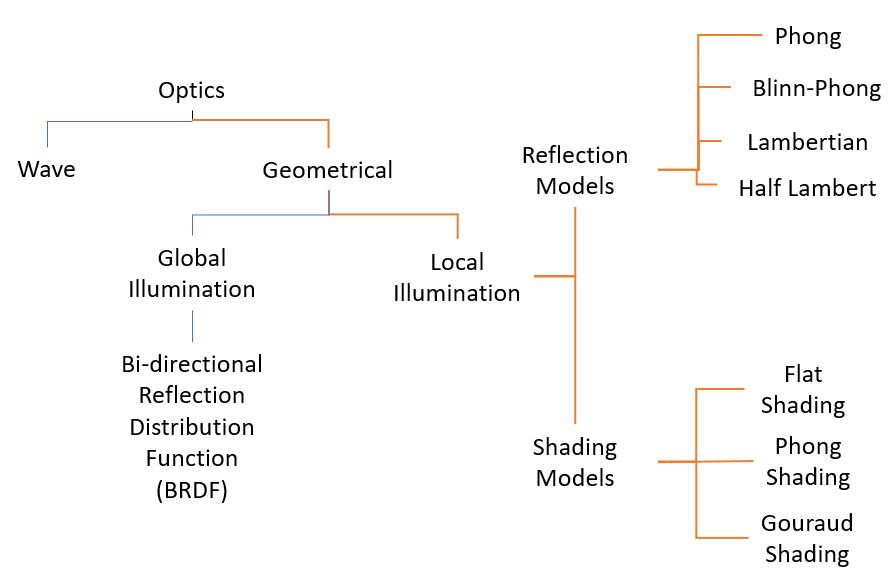
\includegraphics[scale=0.5]{./images/problem-domain-analysis}
	\caption{Problem Domain for Lighting Models of Computer Graphics.}
	\label{fig:prob-domain-analysis}
\end{figure}

\wss{Can you please explain this scope figure?  It looks like you have put some
	great thinking into coming up with it, and it serves an important purpose, 
	but
	the words in the figure are not enough to explain the distinction between 
	the
	different branches.}
\sms{I've added more context to the scoping in this refined section. Let me 
know if it clarifies the scope in a more appropriate way.}

The problem domain for lighting models in computer graphics is obviously broad. 
To simplify this problem we invoke assumptions \aSref{as-geometrical_appx}, 
\aSref{as-illumination}. This allows us to focus on understanding the 
techniques of local illumination (all aspects connected by the orange line in 
\ref{fig:prob-domain-analysis}).

The scope of the family includes geometrical optics simulation of light 
reflection for 3D material objects in a local illumination context. These are 
the types of lighting and shader models that \famname  will implement.

\subsection{Characteristics of Intended Reader}
The intended readers of this document should have understanding of Grade 12 
Physics (particularly Optics) and a undergraduate Level 2 understanding of 
Linear Algebra and Matrix operations.  

\subsection{Organization of Document}
This document is organized in accordance with the CA template for scientific 
computing software provided by Dr. Smith for CAS 741. These templates are based 
on work by \citet{Smith2006}.

\section{General System Description}
This section identifies the interfaces between the system and its environment,
describes the potential user characteristics and lists the potential system
constraints.

\subsection{Potential System Contexts}
There are two system contexts that \famname and its associated library of 
lighting models can be used in, depending on the use case.

\subsubsection{Creator Context}
Figure \ref{fig:system-context} shows the first context, of a user creating 
scenes using the library through the system. The circle represents the system 
user. The box is the library of lighting models system as implemented by 
\famname. Arrows are used to show the flow of data between the system and its 
environment.

\begin{figure}[h]
	\centering
	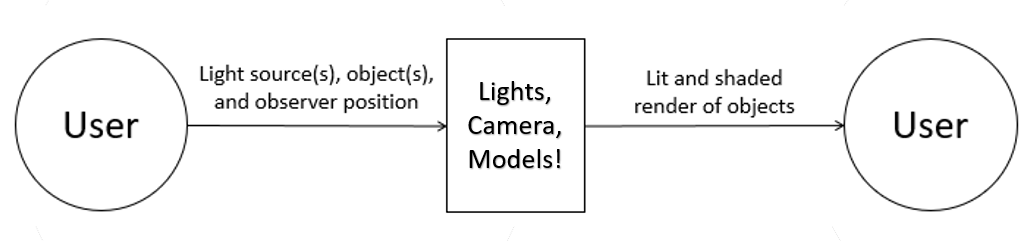
\includegraphics[scale=0.5]{./images/system-context}
	\caption{Creator system context for \famname}
	\label{fig:system-context}
\end{figure}

In this context the responsibilities of the user and system are as follows:
\begin{itemize}
\item User Responsibilities:
	\begin{itemize}
	\item Ensure that the problem they are looking to solve matches the 
	assumptions 
	made for this family.
	\item Provide information on the light source(s), object(s) in scene, and 
	observer position.
	\item Declare shading model to use from preset options.
	\item Declare lighting model to use from present options.
	\item Ensure application programming interface use complies with the user 
	guide.
	\end{itemize}
\item \famname{} Responsibilities:
	\begin{itemize}
	\item Calculate the reflections of all light rays coming from the light 
	source(s).
	\item Determine which light rays (reflected or from source) reach the 
	observer.
	\item Render a lit environment based on selected shading and lighting model.
	\item Update the calculations and render in response to changes in the 
	input 
	data.
	\item Detect data type mismatch, such as a string of characters instead of a
	  floating point number.
	\end{itemize}
\end{itemize}

\subsubsection{Learner Context}
Figure \ref{fig:system-context-2} shows the second context, of a user exploring 
lighting models through manipulating the lighting model, light source, and the 
object's material properties. The circle represents the system user. The box is 
the front-end interface of \famname. Arrows are used to show the flow of data 
between the system and its environment.

\begin{figure}[h]
	\centering
	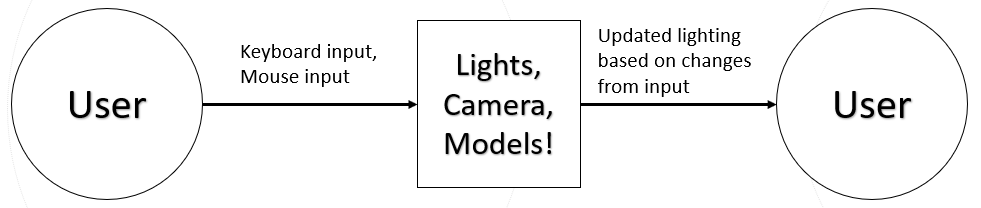
\includegraphics[scale=0.5]{./images/system-context-2}
	\caption{Learner system context for \famname}
	\label{fig:system-context-2}
\end{figure}

The difference between these contexts are the responsibilities of the user and 
system. In this context the responsibilities of the user and system are as 
follows:
\begin{itemize}
	\item User Responsibilities:
	\begin{itemize}
		\item Provide input consistent with the UI statements (keyboard and 
		specific mouse input)
	\end{itemize}
	\item \famname{} Responsibilities:
	\begin{itemize}
		\item Calculate the reflections of all light rays coming from the light 
		source(s).
		\item Determine which light rays (reflected or from source) reach the 
		observer.
		\item Render a lit environment based on selected shading and lighting 
		model.
		\item Update the calculations and render in response to changes in the 
		input data.
	\end{itemize}
\end{itemize}

\subsection{Potential User Characteristics} \label{SecUserCharacteristics}
\subsubsection{Creator Context Users}
The end user of \famname{} should have an Computer Science/Software Engineering 
Undergraduate Level 3 understanding of Computer Graphics (such as through 
completing the SFWR ENG/CS 3GC3) and moderate experience with programming.

\subsubsection{Learner Context Users}
The end user of \famname in this context has no conceptual restraints.

\subsection{Potential System Constraints}
\label{sec:Constraints}
We constrain this system to be implemented in the Unity Engine.
This allows us to focus on exploring the scope of lighting models, as Unity 
will handle the rendering and camera.

%\plt{You may not have any system constraints.}
%\plt{If you need to make design decisions for your family, these decisions will
%  be made here as constraints.  For instance, if all inputs will have to use 
%the
%same file format, this would be a constraint that would be included here.}
%
%\plt{You should generally limit the number of constraints, to keep the CA
%  abstract.}

\section{Commonalities}
This section presents a high-level view of the problem. It captures terminology 
and definitions relevant to the problem, theoretical models that are common to 
all members of the family, goal statements of the family, data definitions that 
will be used to solve these problems, as well as commonalities in inputs, 
calculations, and outputs.

This section also provides a background overview which explains the motivation 
for this work.

\subsection{Background Overview} \label{Sec_Background}
Computer graphics and the techniques developed therein have become extremely 
useful in a variety of fields. Animation, games and media all rely on computer 
graphics to render semi-realistic images for their applications. As we move 
into an era of virtual and augmented reality we see that computer graphics has 
a place beyond the scope of entertainment. Training and rehabilitation 
simulations are extremely popular uses for computer graphics.

Modeling the interaction of light in realistic ways is difficult for computers. 
As such it becomes essential to have mostly accurate approximations of lights 
behaviours that can be used to render scenes in near real-time. On top of the 
need for efficient approximations, it's imperative to make the libraries and 
programs that handle lighting easy to use. It would create an incredibly high 
learning curve if users needed to understand all of the linear algebra and 
physics behind the approximations to mock up a scene. Existing paradigms for 
graphics coding offer APIs to try and make it more user friendly, but there is 
still a disproportionate focucs in graphics to manually fixing the scene and 
matrix manipulations. 

The broad purpose of this work is to abstract the details of lighting in 
computer graphics. We aim for end-users to specify their objects and light 
sources, and have the system render a fully lit and shaded scene. This type of 
work would be useful in teaching lighting model concepts, as it would easily 
allow for switching between different models. More concretely the exercise of 
understanding the family of lighting models would allow for future students to 
review this creation process and have a deeper understanding of lighting in 
computer graphics. Outside of academia, it would similarly be useful for 
individuals working on small scale graphics problems, like prototyping a 
simulation environment. Work like this would allow them to not worry about the 
math involved in getting the environment lit adequately, and instead to focus 
on their more abstract problem.

\subsection{Terminology and  Definitions}
This subsection provides a list of terms that are used in the subsequent
sections and their meaning, with the purpose of reducing ambiguity and making it
easier to correctly understand the requirements. Definitions are borrowed or 
synthesized from \cite{Lengyel2003,Comninos2005,shreiner2012}.

\begin{itemize}
%Physics/Abstract Problem 
\item[\label{}] \textit{Geometrical Optics}: The study of lights as rays.
\item[\label{}] \textit{Ray}: A view of light as a continuous beam, represented 
as a 
vector.
\item[\label{}] \textit{Reflection}: The redirection caused by collision of 
light rays 
with objects.
\item[\label{}] \textit{Specular reflection}: Perfect reflection of a light ray 
on a smooth/glossy surface. This is used to create highlights on objects, or 
create highly reflective objects like mirrors.
\item[\label{}] \textit{Diffuse (Lambertian) reflection}: Reflected light ray 
is scattered in random directions due to microfacets in the surface. This type 
of reflection does not depend of the position of an observer.
\item[\label{}] \textit{Refraction}: The redirection of light rays when passing 
through 
different materials.
%------------Lighting in Graphcis--------------------------------------
\item[\label{}] \textit{Illumination}: Process by which amount of light 
reaching a 
surface is determined.
\item[\label{}] \textit{Global Illumination}: Interactions of light through an 
entire scene as it reflects off of objects onto other objects. Often done 
through techniques like ray tracing, and radiosity.
\item[\label{}] \textit{Ray tracing}: A rendering technique that traces the 
path of light as pixels through a scene and models its interaction with the 
objects it collides with.
\item[\label{}] \textit{Luminous Intensity}: Luminous intensity, or just 
intensity, is the power of the light emitted from a light source. Intensity is 
at its strongest at the light source, and depending on the type of light 
source, will decay with distance.
\item[\label{}] \textit{Local Illumination}: Interactions of light from light 
sources with individual objects as defined by the shading and lighting models.
\item[\label{}] \textit{Shading Model}: methods used to determine the colour 
and intensity of light reflected towards viewer. 
\item[\label{}]\textit{Lighting model}: Method used to calculate the colour of 
a point on a surface. Incorporates a reflection model and a shading model. 
\item[\label{}] \textit{Reflection model}: How light reflects off a surface. 
\item[\label{}] \textit{Shading model}: How the normal vector is calculated for 
polygons in the scene.
%------------Light sources--------------------------------------
\item[\label{}] \textit{Light source}: The origin of light rays.
\item[\label{}] \textit{Ambient light}: Light with no identifiable source or 
direction. It has equal intensity in every direction, and illuminates every 
part of an object uniformly.
\item[\label{}] \textit{Directional (or infinite) light}: Light defined only by 
direction; light travels infinitely in that single direction with constant 
intensity. 
\item[\label{}] \textit{Point light}: Light defined only by a point; light 
travels uniformly in every direction from that point, with intensity decreasing 
with inverse square of distance from source. 
\item[\label{}] \textit{Spotlight}: Light defined by a point and direction; 
light travels infinitely in a single direction from the defined source point 
with intensity decreasing with inverse square of distance from source and 
increased radius of coverage.
%----------------Objects-------------------------------------
\item[\label{}] \textit{Render}: The output of a graphics program.
\item[\label{}] \textit{Environment}: The background objects in a scene along 
with information about light sources.
\item[\label{}] \textit{Scene}: A collection of objects with specific material 
properties. 
\item[\label{}] \textit{Object}: A mesh with material properties that creates a 
three-dimensional shape/object such as a cube, sphere, teapot, etc.
\item[\label{}] \textit{Mesh}: Set of polygons and their associated vertices 
and edges that make up an object.
\item[\label{}]\textit{Surface}: Polygon face of a mesh. 
\item[\label{}] \textit{Polygon}: Closed two-dimensional shape (with well 
defined interior and exterior). Used to define faces of an object on a mesh, 
they are most often triangles, but can be other closed two-dimensional shapes 
as well.
\item[\label{}] \textit{Normal}: A vector perpendicular to a surface, point, or 
pair of vectors.
\item[\label{}]\textit{Surface Normal}: Vector perpendicular to a surface of 
the object's mesh.
\item[\label{} ]\textit{Material Properties}: Properties of the surface of the 
object, including its texture and colour.
\item[\label{}]\textit{Texture}: The quality of a material that determines how 
it reflects light specularly and diffusely.


\end{itemize}

\subsection{Data Definitions} \label{sec_datadef}
This section collects and defines all the data needed to build the instance
models. The dimension of each quantity is also given.

~\newline

\noindent
\begin{minipage}{\textwidth}
\renewcommand*{\arraystretch}{1.5}
\begin{tabular}{| p{\colAwidth} | p{\colBwidth}|}
\hline
\rowcolor[gray]{0.9}
Number& DD\refstepcounter{datadefnum}\thedatadefnum \label{DD_Dot_Product}\\
\hline
Label& \bf Dot Product of two n-dimensional vectors\\
\hline
Symbol &$P\bullet Q$\\
\hline
% Units& $Mt^{-3}$\\
% \hline
  SI Units & --\\
  \hline
  Equation&$P\bullet Q = \sum_{1}^{n}P_{i}Q_{i}$\\
  \hline
  Description & $P$ and $Q$ are two $n$-dimensional vectors. The dot product 
  ($P\bullet Q$) is the scalar sum of the products of each component. The dot 
  product acts a measure of the difference between the directions in which $P$ 
  and $Q$ point. $P$ and $Q$ are perpendicular when $P\bullet Q = 0$..
  \\
  \hline
  Sources& \cite{Lengyel2003}\\
  \hline
  Ref.\ By & \aBref{as-coordinate_system}, \aSref{as-emission_constraint}, 
  \iref{IM_LamDiffuse}, \iref{IM_HalfLam}, \iref{IM_Phong}, 
  \iref{IM_Blinn_Phong}, \tref{TM_Reflection} and \dref{GD_diffReflect}\\
  \hline
\end{tabular}
\end{minipage}\\

~\newline

\noindent
\begin{minipage}{\textwidth}
	\renewcommand*{\arraystretch}{1.5}
	\begin{tabular}{| p{\colAwidth} | p{\colBwidth}|}
		\hline
		\rowcolor[gray]{0.9}
		Number& DD\refstepcounter{datadefnum}\thedatadefnum 
		\label{DD_Cross_Product}\\
		\hline
		Label& \bf Cross Product of two 3-dimensional vectors\\
		\hline
		Symbol &$P\times Q$\\
		\hline
		% Units& $Mt^{-3}$\\
		% \hline
		SI Units & --\\
		\hline
		Equation&$P\times Q = \langle P_{y}Q_{z}-P_{z}Q_{y}, 
		P_{z}Q_{x}-P_{x}Q_{z}, P_{x}Q_{y}-P_{y}Q_{x} \rangle$ 
		
%		\wss{Do
%                          you consistently use angle brackets to define 
%vectors?
%           I think it would be a good idea to include a section in the 
%Reference
%                          Material section that explains your notational 
%conventions.}
          \\
		\hline
		Description & $P$ and $Q$ are two $3$-dimensional vectors. The cross 
		product ($P\times Q$) is the unit vector normal to both $P$ and $Q$. 
		The calculation of the cross product's direction follows the 
		\textit{right hand rule} paradigm. This is used in \tref{TM_Reflection} 
		and \dref{GD_diffReflect}.
		\\
		\hline
		Sources& \cite{Lengyel2003}\\
		\hline
		Ref.\ By & \aBref{as-coordinate_system} \\
		\hline
	\end{tabular}
\end{minipage}\\

~\newline

\noindent
\begin{minipage}{\textwidth}
	\renewcommand*{\arraystretch}{1.5}
	\begin{tabular}{| p{\colAwidth} | p{\colBwidth}|}
		\hline
		\rowcolor[gray]{0.9}
		Number& DD\refstepcounter{datadefnum}\thedatadefnum 
		\label{DD_Intensity_ambient}\\
		\hline
		Label& \bf Ambient Intensity for a Light Source\\
		\hline
		Symbol &$I_{a}$\\
		\hline
		% Units& $Mt^{-3}$\\
		% \hline
		SI Units & cd\\
%-- \wss{I wrote this elsewhere, but shouldn't
%	luminance have units?}		
		\hline
		Equation&$I_{a} = (I_{ar}, I_{ag}, I_{ab}) = i(p,p_{0}) \cdot k_{a}$\\
		\hline
		Description & $i(p, p_{0})$ is the intensity of the light at point $p$ 
		from light source position $p_{0}$. Depending on the type of light 
		source the intensity will change with distance from the source.\\
		& $k_{a}$ is the coefficient of ambient reflection. \\
		\hline
		Sources& \cite{shreiner2012}\\
		\hline
		Ref.\ By & \iref{IM_Phong}, \iref{IM_Blinn_Phong}\\
		\hline
	\end{tabular}
\end{minipage}\\


~\newline

\noindent
\begin{minipage}{\textwidth}
	\renewcommand*{\arraystretch}{1.5}
	\begin{tabular}{| p{\colAwidth} | p{\colBwidth}|}
		\hline
		\rowcolor[gray]{0.9}
		Number& DD\refstepcounter{datadefnum}\thedatadefnum 
		\label{DD_Intensity_diffuse}\\
		\hline
		Label& \bf Diffuse Luminance for a Light Source\\
		\hline
		Symbol &$I_{d}$\\
		\hline
		% Units& $Mt^{-3}$\\
		% \hline
		SI Units & cd\\
		\hline
		Equation&$I_{d} = (I_{dr}, I_{dg}, I_{db})= k_{d}\cdot i(p,p_{0}) \cdot 
		\max(0,(L_{i}\bullet N))$\\
		\hline
		Description & $p$ is the point where $L_{i}$ hits the surface of an 
		object.
		\\
		& $i(p, p_{0})$ is the intensity of $L_{i}$ at point $p$ from light 
		source position $p_{0}$. \\
		& $k_{d}$ is the coefficient of diffuse reflection. \\
		& $L_{i}$ is the incidence ray.\\
		& $N$ is the unit vector surface normal. \\
		\hline
		Sources& \cite{shreiner2012}\\
		\hline
		Ref.\ By & \iref{IM_LamDiffuse}, \iref{IM_HalfLam}, \iref{IM_Phong}, 
		\iref{IM_Blinn_Phong} \\
		\hline
	\end{tabular}
\end{minipage}\\

~\newline

\noindent
\begin{minipage}{\textwidth}
	\renewcommand*{\arraystretch}{1.5}
	\begin{tabular}{| p{\colAwidth} | p{\colBwidth}|}
		\hline
		\rowcolor[gray]{0.9}
		Number& DD\refstepcounter{datadefnum}\thedatadefnum 
		\label{DD_Intensity_specular}\\
		\hline
		Label& \bf Specular Luminance for a Light Source\\
		\hline
		Symbol &$I_{s}$\\
		\hline
		% Units& $Mt^{-3}$\\
		% \hline
		SI Units & cd\\
		\hline
		Equation&$I_{s} = (I_{sr},I_{sg},I_{sb}) = 
		k_{s}\cdot i(p,p_{0}) \cdot \max(0, ({L_{r}}\bullet V))^\alpha$ \\
		\hline
		Description & $p$ is the point where $L_{i}$ hits the surface of an 
		object.
		\\
		& $i(p, p_{0})$ is the intensity of $L_{i}$ at point $p$ from light 
		source position $p_{0}$. \\
		& $L_{r}$ is the reflected ray. It is the reflection of the incidence 
		ray, $L_{i}$, about the normal, $N$.\\
		& $V$ is the unit vector between the point where the incidence ray hit 
		the object, and the observer. \\
		& $k_{s}$ is the specular coefficient of the material.\\
		& $\alpha$ is the shininess coefficient to determine the size of the 
		specular highlight. The following image describes the behaviour of the 
		specular highlight size based on $\alpha$\\
		& 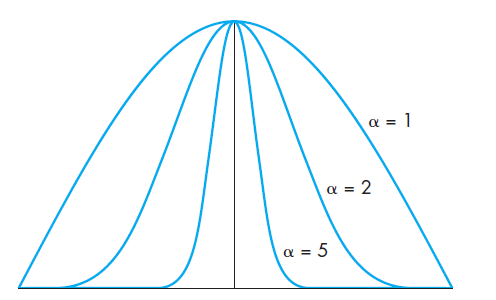
\includegraphics[]{./images/shininess-coefficient}\\
		\hline
		Sources& \cite{shreiner2012}\\
		\hline
		Ref.\ By & \iref{IM_Phong}, \iref{IM_Blinn_Phong}\\
		\hline
	\end{tabular}
\end{minipage}\\

~\newline

\noindent
\begin{minipage}{\textwidth}
	\renewcommand*{\arraystretch}{1.5}
	\begin{tabular}{| p{\colAwidth} | p{\colBwidth}|}
		\hline
		\rowcolor[gray]{0.9}
		Number& DD\refstepcounter{datadefnum}\thedatadefnum 
		\label{DD_Intensity_Total}\\
		\hline
		Label& \bf Total Luminance for a Light Source\\
		\hline
		Symbol &$I_{T}$\\
		\hline
		% Units& $Mt^{-3}$\\
		% \hline
		SI Units & cd\\
		\hline
		Equation&$I_{T} = I_{a} + I_{d} + I_{s}$ \\
		\hline
		Description & Total luminance is the combination of ambient, diffuse, 
		and specular luminance.
		\\
		\hline
		Sources& \cite{shreiner2012}\\
		\hline
		Ref.\ By & \iref{IM_Phong}, \ddref{DD_Intensity_PointSource_Distance} \\
		\hline
	\end{tabular}
\end{minipage}\\

~\newline

\noindent
\begin{minipage}{\textwidth}
	\renewcommand*{\arraystretch}{1.5}
	\begin{tabular}{| p{\colAwidth} | p{\colBwidth}|}
		\hline
		\rowcolor[gray]{0.9}
		Number& DD\refstepcounter{datadefnum}\thedatadefnum 
		\label{DD_Intensity_PointSource_Distance}\\
		\hline
		Label& \bf Luminous intensity at point $p$ from a point source, 
		$p_{0}$\\
		\hline
		Symbol &$i(p, p_{0})$\\
		\hline
		% Units& $Mt^{-3}$\\
		% \hline
		SI Units & cd\\
		\hline
		Equation&$i(p, p_{0}) = \frac{1}{|p-p_{0}|^2} I(p_{0})$\\
		\hline
		Description & Calculates the intensity of light at point $p$ from a 
		light source at position $p_{0}$ in Cartesian Coordinates.\\
		& $I(p_{0})$ is the intensity of the light source at it's source. 
		Therefore it is just the straight intensity of the light, or $I_{T}$.\\
		\hline
		Sources& \cite{Lengyel2003}\\
		\hline
		Ref.\ By & \aBref{as-coordinate_system} \\
		\hline
	\end{tabular}
\end{minipage}\\

~\newline

\noindent
\begin{minipage}{\textwidth}
	\renewcommand*{\arraystretch}{1.5}
	\begin{tabular}{| p{\colAwidth} | p{\colBwidth}|}
		\hline
		\rowcolor[gray]{0.9}
		Number& DD\refstepcounter{datadefnum}\thedatadefnum 
		\label{DD_Flat_Shading}\\
		\hline
		Label& \bf Calculation of Normals for Flat Shading\\
		\hline
		Symbol &$\vec{n}$\\
		\hline
		% Units& $Mt^{-3}$\\
		% \hline
		SI Units & --\\
		\hline
		Equation&$\vec{n} = \frac{\vec{P} \times \vec{Q}}{|\vec{P} \times 
		\vec{Q}|}$\\
		\hline
		Description & Flat shading calculates the surface normal of a polygon 
		in a mesh. Given two non-parallel vectors tangent to the surface of the 
		polygon, $\vec{P}$ and $\vec{Q}$,the normal ($\vec{n}$) is 
		the normalized cross-product of $\vec{P}$ and $\vec{Q}$ \\
		\hline
		Sources& \cite{shreiner2012}\\
		\hline
		Ref.\ By & \aBref{as-coordinate_system} \\
		\hline
	\end{tabular}
\end{minipage}\\

~\newline

\noindent
\begin{minipage}{\textwidth}
	\renewcommand*{\arraystretch}{1.5}
	\begin{tabular}{| p{\colAwidth} | p{\colBwidth}|}
		\hline
		\rowcolor[gray]{0.9}
		Number& DD\refstepcounter{datadefnum}\thedatadefnum 
		\label{DD_Gouraud_Shading}\\
		\hline
		Label& \bf Calculation of Normals for Gouraud Shading\\
		\hline
		Symbol &$\vec{n_{v}}$\\
		\hline
		% Units& $Mt^{-3}$\\
		% \hline
		SI Units & --\\
		\hline
		Equation&$\vec{n_{v}} = 
		\frac{\sum_{i=1}^{t_{v}}n_{i}}{|\sum_{i=1}^{t_{v}}n_{i}|}$\\
		\hline
		Description & Gouraud shading calculates the normal at the vertices of 
		a polygon in a mesh. Given a vertex, $v$,the normal ($\vec{n_{v}}$) is 
		the normalized average of the surface normals ($\vec{n_{i}}$) for all 
		polygons that share that vertex. $t_{v}$ is the number of polygons that 
		share the vertex $v$.\\
		& 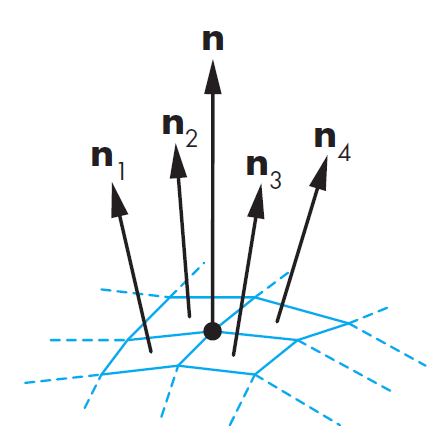
\includegraphics[]{./images/gouraud-shading-interpolation}\\
		\hline
		Sources& \cite{shreiner2012}\\
		\hline
		Ref.\ By & \aBref{as-coordinate_system}\\
		\hline
	\end{tabular}
\end{minipage}\\

~\newline

\wss{You talk about surfaces, and polygons, but I don't see how you actually
  represent an object.  Searching through again, I see that objects have a set
  of possible shapes, but I don't see the connection between the shapes and
  polygons.  The shapes are mathematical defined, especially something like a
  sphere or a cube.  I think you need to say somewhere that you approximate the
  shape with a mesh of polygons.  You might want to look at the commonality
  analysis of mesh generators that I wrote with a student years ago.  It should
  be in our cas741 repo under CAS 04-10-SS.pdf.}
\sms{I was under the impression that "how" I represent an object is too design 
	specific for a CA. I've modified the definitions of "Object" to describe it 
	as a mesh with material properties that forms a 3d-shape, and re-specified 
	polygons as being closed 2d-shapes used to define object surfaces on the 
	mesh. Is this a sufficient explanation?}

\noindent
\begin{minipage}{\textwidth}
	\renewcommand*{\arraystretch}{1.5}
	\begin{tabular}{| p{\colAwidth} | p{\colBwidth}|}
		\hline
		\rowcolor[gray]{0.9}
		Number& DD\refstepcounter{datadefnum}\thedatadefnum 
		\label{DD_Phong_Shading}\\
		\hline
		Label& \bf Calculation of Normals for Phong Shading\\
		\hline
		Symbol &$\vec{n_{v}}$\\
		\hline
		% Units& $Mt^{-3}$\\
		% \hline
		SI Units & --\\
		\hline
		Equation& \\
		\hline
		Description & Phong shading linearly interpolates normals across each 
		the surface of the polygon from the vertex normals. Surface normals are 
		then normalized per pixel.\\
		& 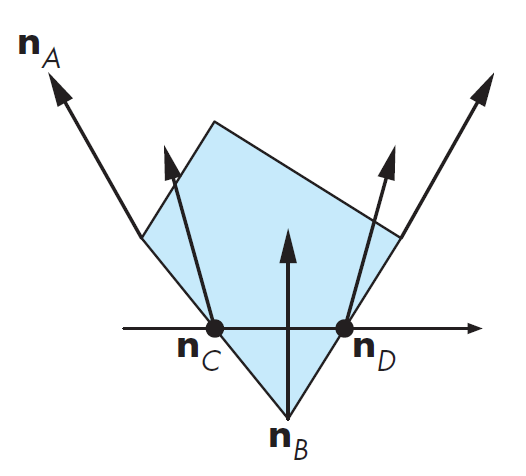
\includegraphics[]{./images/phong-shading-interpolation} \\
		\hline
		Sources& \cite{shreiner2012}\\
		\hline
		Ref.\ By & \aBref{as-coordinate_system}, \aBref{as-coordinates} \\
		\hline
	\end{tabular}
\end{minipage}\\


\subsection{Goal Statements}

\noindent Given some light source(s), some object(s) and their respective 
material properties, and an observer the goal statements are:

\begin{itemize}

\item[GS\refstepcounter{goalnum}\thegoalnum \label{gs-display}:] 
Render a fully lit and shaded scene of the objects based on the observer 
location.

\end{itemize}

There are two components to achieving this goal: 
\begin{itemize}
	\item calculating the lighting of the scene based on the light, object, and 
	lighting model, and
	\item rendering the scene based on those calculations and the observer 
	location
\end{itemize}

The rendering of the scene will be handled by the Unity Engine, as stated in 
our System Constraints \ref{sec:Constraints}. This means that this document 
will concern itself with refining the methods of calculation of lighting for 
the scene.

\wss{I like this goal statement.  However, I feel like the rest of the document
	doesn't completely refine it.  I feel like there should be an instance model
	that takes the refined version of these inputs and outputs a refined version
	of the output.}\\
\sms{The larger issue is that the rendering aspect is out of scope of the 
problem we previously defined (the lighting models). I've added more context to 
the goal statement to explain that this is basically a two stage goal, one of 
which is handled by the system I am designing, the other is handled by the 
Unity Engine.}

\subsection{Theoretical Models} \label{sec_theoretical}

This section focuses on the general equations and laws that \famname{} is based
on.  %\plt{Modify the examples below for your problem, and add additional models
%  as appropriate.}

~\newline

\noindent
\begin{minipage}{\textwidth}
\renewcommand*{\arraystretch}{1.5}
\begin{tabular}{| p{\colAwidth} | p{\colBwidth}|}
  \hline
  \rowcolor[gray]{0.9}
  Number& T\refstepcounter{theorynum}\thetheorynum \label{TM_Reflection}\\
  \hline
  Label&\bf Law of Reflection\\
  \hline
  Equation&   $\theta_{i} = \theta_{r}$ or 
  $L_{i}\bullet N = 
  L_{r} \bullet N$\\
  \hline
  Description & 
                When a ray of light reflects off a surface, the angle of 
                incident is equal to the angle of reflection. This can also be 
                written as the dot product of the incident ray and the normal 
                is equal to the dot product of the reflected ray and the 
                normal.
		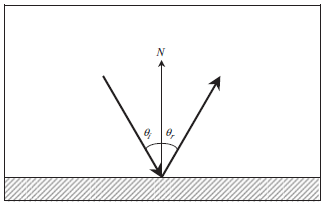
\includegraphics[scale=1]{./images/specular-reflection}  
		\\              
                                
  \hline
  Source & \cite{Comninos2005}\\
  \hline
  Ref.\ By & \dref{GD_diffReflect}\\
  \hline
\end{tabular}
\end{minipage}\\

~\newline

%\plt{In a CA, the TMs often do not need to be refined.  However, this is not a
%  rule.  In some cases, it may make sense to introduce an IM, or possibly even 
%a
%  GD in between the TM and the IM.}

\subsubsection{General Definitions}\label{sec_gendef}

%\plt{General Definitions (GDs) are a refinement of one or more TMs, and/or of
%	other GDs.  The GDs are less abstract than the TMs.  Generally the reduction
%	in abstraction is possible through invoking (using/referencing) Assumptions.
%	For instance, the TM could be Newton's Law of Cooling stated abstracting.  
%	The GD could take the general law and apply it to get a 1D equation.}

This section collects the laws and equations that will be used in building the
instance models.

%\plt{Some projects may not have any content for this section, but the section
%	heading should be kept.}  \plt{Modify the examples below for your problem, 
%	and
%	add additional definitions as appropriate.}

~\newline

\noindent
\begin{minipage}{\textwidth}
	\renewcommand*{\arraystretch}{1.5}
	\begin{tabular}{| p{\colAwidth} | p{\colBwidth}|}
		\hline
		\rowcolor[gray]{0.9}
		Number& GD\refstepcounter{defnum}\thedefnum \label{GD_diffReflect}\\
		\hline
		Label &\bf Diffuse Reflection \\
		\hline
		% Units&$MLt^{-3}T^0$\\
		% \hline
		SI Units& - \\
		\hline
		Equation& $ \theta_{i} = \theta_{r}$ or 
		$L_{i}\bullet N = 
		L_{r} \bullet N$  \\
		\hline
		Description &
		Law of Reflection applied to rough surfaces.
		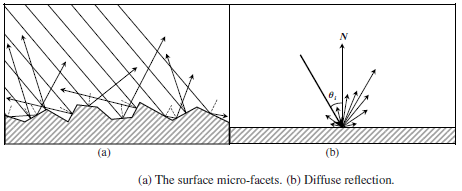
\includegraphics[scale=1]{./images/diffuse-reflection}
		\\
		\hline
		Source & \cite{Comninos2005} \\
		\hline
		Ref.\ By & \ddref{DD_Dot_Product}\\
		\hline
	\end{tabular}
\end{minipage}\\

\section{Variabilities}
The follow section outlines variabilities between family members. Section 
\ref{sec_Assumptions} covers the assumptions made to simplify/realise the 
problem. Section \ref{sec_Calculation} captures variabilities in the 
implementation.

Before tackling those sections, we summarize here variabilities in the problem.

\subsection{Assumptions} \label{sec_Assumptions}
This section outlines the various assumptions made in defining this problem.   
The nature of these assumptions is to make decisions in regards to the 
variabilities of the system. These are invoked to limit the scope of the 
problem being modeled, and often indicate areas where likely changes may occur.

Assumptions are divided based on their binding time. All assumptions are used 
to refine the \gsref{gs-display} and define the potential members of the 
family that will be built.

\subsubsection{Scope Time Bindings}
These assumptions are applied in the abstract design of the program. They 
dictate the family members that we cover, and the potential design choices 
available to us. Changing these assumptions changes the underlying problem; as 
such this would change the family we are discussing. Therefore these 
assumptions will not change, and apply to all members of this family.

~\newline
\textbf{\emph{Physics Assumptions}}
\begin{itemize}
	\item[AS\refstepcounter{assumpnumS}\theassumpnumS\label{as-geometrical_appx}:]
	Light interactions will be defined by Geometrical Optics principles 
	(ray-based).
\end{itemize}

~\newline
\textbf{\emph{Rendering Limitations}}
\begin{itemize}
	\item[AS\refstepcounter{assumpnumS}\theassumpnumS\label{as-illumination}:]
	Lighting will be handled at the local illumination level.
\end{itemize}

\subsubsection{Build Time Bindings}
These assumptions are applied in the concrete design of any individual family 
member. They dictate the specifics of that family member, and concretize our 
design choices. Changing these assumptions would change the particular family 
member that is being built. As such, these assumptions are likely to change for 
different contexts.

~\newline
\textbf{\emph{Scene Assumptions}}
\begin{itemize}
	\item[AB\refstepcounter{assumpnumB}\theassumpnumB\label{as-coordinate_system}:]
	The virtual environment will be described by a 3D Caretsian Coordinate 
	System using right-hand rules.
	\begin{itemize}
		\item[] \textit{Alternate Assumptions}
		\begin{itemize}
			\item The virtual environment will be described by a polar 
			coordinate system.
		\end{itemize}
	\end{itemize}
	\item[AB\refstepcounter{assumpnumB}\theassumpnumB\label{as-number-scenes}:]
	Only one scene can be loaded into the system at a time.
	\item[AB\refstepcounter{assumpnumB}\theassumpnumB\label{as-scenes-size}:]
	The scene size is defined as a rectangular room with dimensions 
	SCENE\_HEIGHT, SCENE\_WIDTH, and SCENE\_DEPTH.
\end{itemize}

~\newline
\textbf{\emph{Object Assumptions}}
\begin{itemize}
	\item[AB\refstepcounter{assumpnumB}\theassumpnumB\label{as-object-opaque}:] 
	All objects are opaque; light will not experience refraction with any 
	object. 
	\begin{itemize}
		\item[] \textit{Alternate Assumptions}
		\begin{itemize}
			\item Objects can be transparent or opaque; light will experience 
			refraction with transparent objects.
			\item Objects can be transparent, translucent, or opaque; light 
			will experience refraction with transparent and translucent objects.
		\end{itemize}
	\end{itemize}	
	\item[AB\refstepcounter{assumpnumB}\theassumpnumB\label{as-loc-vs-global}:]
	Objects will not cast shadows on each other. Related to 
	\aSref{as-illumination}.	
	\item[AB\refstepcounter{assumpnumB}\theassumpnumB\label{as-illum_constraint}:]
	Objects will not reflect light at each other. Related to 
	\aSref{as-illumination}.
	\item[AB\refstepcounter{assumpnumB}\theassumpnumB\label{as-emission_constraint}:]
	Objects will not emit light. Related to \aSref{as-illumination}.
	\item[AB\refstepcounter{assumpnumB}\theassumpnumB\label{as-obj-coord}:]
	Positions of objects are defined on a 3D Cartesian Coordinate System. 
	Related to \aBref{as-coordinate_system}.
	\item[AB\refstepcounter{assumpnumB}\theassumpnumB\label{as-obj-pos}:]
	Objects have a fixed position and will not be moved during the running of 
	the program.
	\item[AB\refstepcounter{assumpnumB}\theassumpnumB\label{as-object_mesh}:] 
	Object shapes will be approximated by a polygon mesh of triangles.
	\begin{itemize}
		\item[] \textit{Alternate Assumptions}
		\begin{itemize}
			\item Objects will be approximated by a polygon mesh of 
			quadrilaterals.
			\item Objects will be approximated by a polygon mesh of convex 
			polygons.
		\end{itemize}
	\end{itemize}			
	\item[AB\refstepcounter{assumpnumB}\theassumpnumB\label{as-poly-mesh-store}:]
	Object polygon mesh is stored as a list of vertices and a set of polygon 
	surfaces that are associated with vertices. Related to 
	\aBref{as-object_mesh}.
	\begin{itemize}
		\item[] \textit{Alternate Assumptions}
		\begin{itemize}
			\item Polygon mesh is stored as list of all vertices, and edges 
			connecting them.
		\end{itemize}
	\end{itemize}		
	\item[AB\refstepcounter{assumpnumB}\theassumpnumB\label{as-object_representation2}:]
	Object meshes will be closed and convex (there is a well defined interior 
	and exterior). Related to \aBref{as-object_mesh}
\end{itemize}

~\newline
\textbf{\emph{Lighting Assumptions}}
\begin{itemize}
	\item[AB\refstepcounter{assumpnumB}\theassumpnumB\label{as-light-coord}:]
	Positions of light sources are defined on a 3D Cartesian Coordinate System. 
	Related to \aBref{as-coordinate_system}.
	\item[AB\refstepcounter{assumpnumB}\theassumpnumB\label{as-light-fixed}:]
	Light sources have a fixed position and will not be moved during the 
	running of the program.	Related to \aBref{as-light-coord}.
\end{itemize}

~\newline
\textbf{\emph{Observer Assumptions}}
\begin{itemize}
	\item[AB\refstepcounter{assumpnumB}\theassumpnumB\label{as-obsv_total}:]
	There will only be a single observer in a scene.
	\item[AB\refstepcounter{assumpnumB}\theassumpnumB\label{as-obsv-coord}:]
	Observer position is defined on a 3D Cartesian Coordinate System. 
	Related to \aBref{as-coordinate_system}.
	\item[AB\refstepcounter{assumpnumB}\theassumpnumB\label{as-obsv_move}:]
	The observer position will be fixed for the run-time of the program.
\end{itemize}

~\newline
\textbf{\emph{Input Assumptions}}
\begin{itemize}
	\item[AB\refstepcounter{assumpnumB}\theassumpnumB\label{as-input-format}:]
	Input will be accepted as a formatted JSON file.
\end{itemize}

\subsubsection{Run Time Bindings}
These assumptions are used to detail the specifics of the individual program 
that will run. Most of these are captured as inputs to the system. These can 
change as the program is developed.

~\newline
\textbf{\emph{Lighting Assumptions}}
\begin{itemize}
	\item[AR\refstepcounter{assumpnumR}\theassumpnumR\label{as-light-num}:]
	There will be only one light source in the scene.
	\begin{itemize}
		\item[] \textit{Alternate Assumptions}
		\begin{itemize}
			\item There will be between MIN\_NUM\_LIGHTS and MAX\_NUM\_LIGHTS 
			in the scene.
		\end{itemize}
	\end{itemize}		
	\item[AR\refstepcounter{assumpnumR}\theassumpnumR\label{as-light-type}:]
	The light source will one of the following types: point, spot light, 
	directional, or ambient.
	\item[AR\refstepcounter{assumpnumR}\theassumpnumR\label{as-light-init-pos}:]
	The light source will be positioned at LIGHT\_POSITION.	
	\item[AR\refstepcounter{assumpnumR}\theassumpnumR\label{as-light-overlap}:]
	The LIGHT\_POSITION will not overlap with the OBSERVER\_POSITION or any 
	OBJECT\_POSITION.
	\item[AR\refstepcounter{assumpnumR}\theassumpnumR\label{as-light-colour}:]
	The light source will have a colour defined by an (r,g,b)-tuple called 
	LIGHT\_COLOUR.
	\item[AR\refstepcounter{assumpnumR}\theassumpnumR\label{as-light-default-colour}:]
	The light source colour will default to white (255,255,255) if not 
	specified.
	
\end{itemize}

~\newline
\textbf{\emph{Objects Assumptions}}
\begin{itemize}
	\item[AR\refstepcounter{assumpnumR}\theassumpnumR\label{as-obj-num}:]
	There will be only one object in the scene.
	\begin{itemize}
		\item[] \textit{Alternate Assumptions}
		\begin{itemize}
			\item There will be between MIN\_NUM\_OBJECTS and MAX\_NUM\_OBJECTS 
			in the scene.
		\end{itemize}
	\end{itemize}		
	\item[AR\refstepcounter{assumpnumR}\theassumpnumR\label{as-obj-type}:]
	The object will one of the following types: sphere, cube, torus, or teapot.
	\item[AR\refstepcounter{assumpnumR}\theassumpnumR\label{as-obj-init-pos}:]
	The object will be positioned at OBJECT\_POSITION.
	\item[AR\refstepcounter{assumpnumR}\theassumpnumR\label{as-obj-overlap}:]
	The OBJECT\_POSITION will not overlap with the OBSERVER\_POSITION  or 
	LIGHT\_POSITION.		
	\item[AR\refstepcounter{assumpnumR}\theassumpnumR\label{as-obj-properties}:]
	The object will have values for the reflection, specular, diffuse, and 
	shininess coefficients of its material.
	\item[AR\refstepcounter{assumpnumR}\theassumpnumR\label{as-obj-colour}:]
	The object will have a colour defined by an (r,g,b)-tuple called 
	OBJECT\_COLOUR.
	\item[AR\refstepcounter{assumpnumR}\theassumpnumR\label{as-obj-default-colour}:]
	The object colour will default to white (255,255,255) if not specified.	
\end{itemize}

~\newline
\textbf{\emph{Observer Assumptions}}
\begin{itemize}
	\item[AR\refstepcounter{assumpnumR}\theassumpnumR\label{as-obsv-pos}:]
	The observer will be positioned at OBSERVER\_POSITION.
	\item[AR\refstepcounter{assumpnumR}\theassumpnumR\label{as-obsv-overlap}:]
	The OBSERVER\_POSITION will not overlap with any OBJECT\_POSITION or 
	LIGHT\_POSITION.
\end{itemize}

\wss{The scope time bindings make sense, but I am not sure how to interpret the
  building time bindings.  Since they are build time, I'm assuming that whether
  they apply or not is a build time decision.  Is this correct?  If so, it 
feels like if the assumptions do not apply another assumption will have to take 
its place, but I don't know what that assumption is.  For instance, if the 
object is not represented by a mesh of triangles, what is it represented by?}\\
\sms{Do the changes to the presentation of the assumptions address this issue?}

\wss{I see the connection between the objects and their representation by
  polygons is given here.  I mentioned this in an earlier comment, but I had
  missed this mention.  However, I think you still need more information.  What
  does it mean to represent an object by a mesh?  In the mesh generator CA that
  I mentioned in an earlier comment a mesh is defined as covering up of a
  domain, with several rules.  You might want to look at that definition.}\\
\sms{See response to previous comments.}

\wss{Is the dimension of the problem a variability, or are lighting problems in
  3D?}\\
\sms{I made the scope decision in the introduction that we are only dealing 
with 3D lighting and that these models are specific to 3D lighting. I've tried 
to clarify this again in the expanded scope section.}

\subsection{Calculation} \label{sec_Calculation}
This section outlines variabilities in design details, capturing variabilities 
in: input, calculations, algorithms, and data structures.

~\newline
\textbf{Input variabilities:} 
\begin{table}[H]
	\centering
	\begin{tabular}{|p{3cm}|p{3cm}|p{5cm}|p{2cm}|}
		\hline
		\textbf{Variability} & \textbf{Parameter of Variation} & 
		\textbf{Constraints} &  \textbf{Related} \\
		\hline
		\multirow{3}{*}{Scene Size} & SIZE\_HEIGHT $\in \mathbb{R}$ & $0 \ll$ 
		SIZE\_HEIGHT $\le$ MAX\_HEIGHT & 
		\\
		& SIZE\_WIDTH $\in \mathbb{R}$ & $0 \ll$ 
		SIZE\_WIDTH $\le$ MAX\_WIDTH \wss{The types don't
			match.  You have a
			vector? tuple? of 3
			real numbers for the
			size of the room, but
			the parameters of
			variation is a set of
			real numbers.} \sms{I had read the parameter of variation as 
			telling us the type of that parameter.}& 
			\aBref{as-coordinate_system}\\
		& SIZE\_DEPTH $\in \mathbb{R}$ & $0 \ll $ 
		SIZE\_DEPTH $\le$ MAX\_DEPTH & \aBref{as-scenes-size} \\
		\hline
		\multirow{5}{3cm}{Position of light source (x,y,z)} & x $\in 
		\mathbb{R}$ 
		& 
		$0 \ll x \le$ SIZE\_HEIGHT	& \aRref{as-light-init-pos}\\
		& y $\in \mathbb{R}$ &  $0 \ll y \le$ SIZE\_WIDTH & 
		\aRref{as-light-num}\\
		& z $\in \mathbb{R}$ &  $0 \ll z \le$ SIZE\_DEPTH \wss{The same comment 
		as 
		above applies.}& \aBref{as-light-coord} 
		\\
		& & (x,y,z) $\ne$ OBSERVER\_POSITION & 
		\aBref{as-light-fixed}\\
		& &  (x,y,z) $\ne$ OBJECT\_POSITION & \aRref{as-light-overlap}\\
		\hline		
	\end{tabular}
	\caption{Parameters of Variation for Input (continued).}
	\label{tbl:Input_Variations}
\end{table}

\begin{table}[H]
	\centering
	\begin{tabular}{|p{3cm}|p{3cm}|p{5cm}|p{2cm}|}
		\hline
		\textbf{Variability} & \textbf{Parameter of Variation} & 
		\textbf{Constraints} &  \textbf{Related} \\
		\hline
		\multirow{5}{3cm}{Position of object(s) (x,y,z)} & x$\in \mathbb{R}$ & 
		$0 \ll x \le$ SIZE\_HEIGHT\\
		&  y $\in \mathbb{R}$ & $0 \ll y \le$ SIZE\_WIDTH & 
		\aBref{as-coordinate_system}\\
		& z $\in \mathbb{R}$ &  $0 \ll z \le$ SIZE\_DEPTH & 
		\aRref{as-obj-overlap}\\
		& & (x,y,z) $\ne$OBSERVER\_POSITION &  \\
		& & (x,y,z) $\ne$ LIGHT\_POSITION &  \\
		\hline
		\multirow{5}{3cm}{Position of Observer (x,y,z)} & x $\in \mathbb{R}$ & 
		$0 \ll x \le$ SIZE\_HEIGHT\\
		&  y $\in \mathbb{R}$ & $0 \ll y \le$ SIZE\_WIDTH & 
		\aBref{as-coordinate_system}\\
		& z $\in \mathbb{R}$ &  $0 \ll z \le$ SIZE\_DEPTH & 
		\aRref{as-obsv-overlap} \\
		& & (x,y,z) $\ne$ OBJECT\_POSITION& \\
		& & (x,y,z) $\ne$ LIGHT\_POSITION&  \\
		\hline				
		\multirow{3}{3cm}{Colour of light (r,g,b)} & r $\in \mathbb{Z}$& $0 \le 
		r 
		\le 255$ & --\\
		& g $\in \mathbb{Z}$& $0 \le g \le 255$  \wss{Why not just define a type
		for the integers between 0 and 256?  A similar comment applies 
		elsewhere in this table.} & \iref{IM_LamDiffuse}, 
		\iref{IM_HalfLam}, \iref{IM_Phong}, \iref{IM_Blinn_Phong}  \\\\
		& b $\in \mathbb{Z}$& $0 \le b \le 255$ & \iref{IM_LamDiffuse}, 
		\iref{IM_HalfLam}, \iref{IM_Phong}, \iref{IM_Blinn_Phong}  \\\\
		\hline
		\multirow{3}{3cm}{Colour of object (r,g,b)} & r $\in \mathbb{Z}$& $0 
		\le 
		r \le 255$ & \iref{IM_LamDiffuse}, 
		\iref{IM_HalfLam}, \iref{IM_Phong}, \iref{IM_Blinn_Phong}  \\\\
		& g $\in \mathbb{Z}$& $0 \le g \le 255$ & \iref{IM_LamDiffuse}, 
		\iref{IM_HalfLam}, \iref{IM_Phong}, \iref{IM_Blinn_Phong}  \\\\
		& b $\in \mathbb{Z}$& $0 \le b \le 255$ & \iref{IM_LamDiffuse}, 
		\iref{IM_HalfLam}, \iref{IM_Phong}, \iref{IM_Blinn_Phong}  \\\\
		\hline
	\end{tabular}
	\caption{Parameters of Variation for Input (continued).}
	\label{tbl:Input_Variations_cont}
\end{table}

\begin{table}[H]
	\centering
	\begin{tabular}{|p{3cm}|p{3cm}|p{5cm}|p{2cm}|}
		\hline
		\textbf{Variability} & \textbf{Parameter of Variation} & 
		\textbf{Constraints} &  \textbf{Related} \\
		\hline
		Ambient coefficient of material	& $k_{a} \in \mathbb{R}$ & $0 \le 
		k_{a} \le 1$ & \ddref{DD_Intensity_ambient}, \iref{IM_LamDiffuse}, 
		\iref{IM_HalfLam}, \iref{IM_Phong}, \iref{IM_Blinn_Phong}  \\
		\hline		
		Specular coefficient of material & $k_{s} \in \mathbb{R}$ & $0 \le 
		k_{s} \le 1$ & \ddref{DD_Intensity_specular}, \iref{IM_Phong}, 
		\iref{IM_Blinn_Phong} \\
		\hline
		Diffuse coefficient of material	& $k_{d} \in \mathbb{R}$ & $0.5 \le 
		k_{d} 
		\le 1$ & \ddref{DD_Intensity_diffuse}, \iref{IM_LamDiffuse}, 
		\iref{IM_HalfLam}, \iref{IM_Phong}, \iref{IM_Blinn_Phong}  \\
		\hline		
		Shininess coefficient of material	& $\alpha \in
		\mathbb{Z^{+}}$ & 
		-- & 
		\ddref{DD_Intensity_specular}, \iref{IM_Phong}, \iref{IM_Blinn_Phong} 
		\\
		\hline
		Type of light source & One of \{Point, Spot, Directional, Ambient\} & 
		-- 
		& --\\
		\hline
		Type of object(s) & One of \{Sphere, Cube, Torus, Teapot\} & -- & 
		--\\
		\hline
		Type of shading & One of \{Flat, Gouraud, Phong\} & -- & 
		--\\
		\hline
		Number of object(s) & $\mathbb{R}$ & MIN\_NUM\_LIGHTS $\le$ Number of 
		object(s) $\le$ MAX\_NUM\_OBJECTS & 
		--\\
		\hline
		Number of light(s) & $\mathbb{R}$ & MIN\_NUM\_LIGHTS $\le$ Number of 
		light(s) $\le$ MAX\_NUM\_LIGHTS & 
		--\\
		\hline
		Number of observer(s) & $\mathbb{R}$ & Number of observer(s) $= 
		1$  & 
		--\\
		\hline
		Input method & Single file with light, object and other data; multiple 
		files (one for lights and one for objects) & -- & 
		--\\
		\hline					
	\end{tabular}
	\caption{Parameters of Variation for Input (continued).}
	\label{tbl:Input_Variations_cont2}
\end{table}

~\newpage
\textbf{Calculation variabilities:}
\begin{table}[H]
	\centering
	\begin{tabular}{|p{5cm}|p{5cm}|p{2cm}|p{2cm}|}
		\hline
		\textbf{Variability} & \textbf{Parameters of Variation} & Constraints & 
		\textbf{Ref.}\\
		\hline
		Interpolation of normals for shading & One of 
		$\{$\ddref{DD_Flat_Shading}, \ddref{DD_Gouraud_Shading}, 
		\ddref{DD_Phong_Shading}$\}$ & -- & \aSref{as-coordinate_system} \\
		\hline		
	\end{tabular}
	\caption{Parameters of Variation in Calculations.}
\end{table}

\subsubsection{Instance Models} \label{sec_instance}    

This section transforms the problem defined in 
Section~\ref{sec_problem_definition} into one which is expressed in 
mathematical terms. It uses concrete symbols defined in 
Section~\ref{sec_datadef} to replace the abstract symbols in the models 
identified in Sections~\ref{sec_theoretical} and~\ref{sec_gendef}.

~\newline

%Instance Model 1

\noindent
\begin{minipage}{\textwidth}
	\renewcommand*{\arraystretch}{1.5}
	\begin{tabular}{| p{\colAwidth} | p{\colBwidth}|}
		\hline
		\rowcolor[gray]{0.9}
		Number& IM\refstepcounter{instnum}\theinstnum \label{IM_LamDiffuse}\\
		\hline
		Label& \bf Lambertian (Diffuse) Reflection Model\\
		\hline
		\multirow{7}{*}{Input}& $L_{i}$ : Vector $\langle x, y, z \rangle$ \\
		& $p_{0}$ : Point (x, y, z) \\
		& LIGHT\_COLOUR : (r,g,b)\\
		& $p$ : Point (x,y,z) \\ 
		& OBJECT\_BASE\_COLOUR : (r,g,b)\\
		& $N$ : Vector $\langle x, y, z \rangle$ \\
		\hline
		\multirow{2}{*}{Output}& OBJECT\_RENDERING\_COLOUR : (r,g,b) \\
		\hline
		Equation & $OBJECT\_RENDERING\_COLOUR = 
		((L_{i} \bullet 
		N)(I_{L_{i}p})\cdot(LIGHT\_COLOUR)\cdot(OBJECT\_BASE\_COLOUR)$
		 \\
		\hline
		\multirow{7}{*}{Description} & The Lambertian Reflection Model 
		considers only the 
		diffuse elements of light when calculating the lighting model. The 
		approximation is assuming there's no specular component. This is a 
		refinement on \dref{GD_diffReflect}.\\
		& $L_{i}$ is the vector representation of the incident 
		ray.\\
		& $p$ is the point the incident ray intercepts the surface of an 
		object. \\
		& $p_{0}$ is position of the light source. \\		
		& $N$ is the surface normal unit vector of the object at the position 
		$p$. \\
		& $I_{L_{i}p}$ is the intensity of the light at point $p$, 
		calculated by invoking \ddref{DD_Intensity_PointSource_Distance}, 
		$i(p, p_{0})$\\
		\hline
		Sources& \cite{Comninos2005,Lengyel2003,shreiner2012} \\
		\hline
		Ref.\ By & \iref{IM_HalfLam}\\
		\hline
		Uses & \ddref{DD_Intensity_PointSource_Distance}, 
		\ddref{DD_Dot_Product}\\
		\hline		
	\end{tabular}
\end{minipage}\\

\wss{As Peter pointed out on GitHub, the instance models are incomplete.  Think
  about refining the inputs and outputs.  Including type information with the
  inputs could help.  In particular, object is still vague at this point, and
  you need it to be precise before you can do a calculation.  How the outputs
  are calculated is also needed.}  ~\newline
\sms{Addressed along with the issue on GitHub}

\noindent
\begin{minipage}{\textwidth}
	\renewcommand*{\arraystretch}{1.5}
	\begin{tabular}{| p{\colAwidth} | p{\colBwidth}|}
		\hline
		\rowcolor[gray]{0.9}
		Number& IM\refstepcounter{instnum}\theinstnum \label{IM_HalfLam}\\
		\hline
		Label& \bf Mod Lambert (Diffuse Wrap) Reflection Model\\
		\hline
		\multirow{6}{*}{Input}& $L_{i}$ : Vector $\langle x, y, z \rangle$\\
		& $p$ : Point (x,y,z)\\
		& OBJECT\_BASE\_COLOUR : (r,g,b)\\
		& $k_{d}$ : $\mathbb{R}$ \\
		& LIGHT\_COLOUR : (r,g,b)\\
		& $p_{0}$ : Point (x,y,z) \\
		& $N$ : Vector $\langle x, y ,z \rangle$ \\
		\hline
		Output&  OBJECT\_RENDER\_COLOUR : (r,g,b)\\
		\hline
		\multirow{2}{*}{Equation} & OBJECT\_RENDER\_COLOUR $= 
		(LambertTerm)\cdot$\\
		& (OBJECT\_BASE\_COLOUR)$\cdot$(LIGHT\_COLOUR)$\cdot(I_{L_{i}p})$\\
		\hline
		Description & This is a refinement of \iref{IM_LamDiffuse}. We 
		incorporate the idea of a coefficient of diffuse reflection to modify 
		the sharpness of the shadows. When $k_{d} = 1$ this model acts like 
		\iref{IM_LamDiffuse}. We limit modifications be constraining $k_{d} \ge 
		0.5$; this keeps the shadows visible and conceptually matches the idea 
		that all objects have some element of diffuse reflection. When $k_{d} = 
		0.5$ we call this special case the Half-Lambert Model. \\
		& The $LambertTerm$ is the modified diffuse reflection. It is defined 
		by: $LambertTerm = [(N \bullet L_{i})\cdot k_{d} + (1-k_{d})]^2$\\
		&  $L_{i}$ is the vector representation of the incident 
		ray.\\
		& $N$ is the surface normal unit vector of the object at position 
		$p$. \\
		& $k_{d}$  is the coefficient of diffuse reflection.\\
		& $p$ is the point the incident ray intercepts the surface of an 
		object. \\
		& $p_{0}$ is position of the light source. \\				
		& $I_{L_{i}p}$ is the intensity of the light at point $p$, 
		calculated by invoking \ddref{DD_Intensity_PointSource_Distance}, 
		$i(p, p_{0})$\\
		\hline
		Sources& \cite{Comninos2005,Lengyel2003,shreiner2012} \\
		\hline
		Ref.\ By & -- \\
		\hline
		Uses & \ddref{DD_Intensity_PointSource_Distance}, 
		\ddref{DD_Dot_Product}\\
		\hline
	\end{tabular}
\end{minipage}\\

~\newline

\noindent
\begin{minipage}{\textwidth}
	\renewcommand*{\arraystretch}{1.5}
	\begin{tabular}{| p{\colAwidth} | p{\colBwidth}|}
		\hline
		\rowcolor[gray]{0.9}
		Number& IM\refstepcounter{instnum}\theinstnum \label{IM_Phong}\\
		\hline
		Label& \bf Phong Reflection Model\\
		\hline
		\multirow{12}{*}{Input} & $L_{i}$ : Vector $\langle x, y ,z \rangle$\\
		& $p$ : Point (x,y,z)\\
		& OBSERVER\_POSITION : Point (x,y,z)\\		
		& OBJECT\_POSITION : Point (x,y,z)\\
		& OBJECT\_BASE\_COLOUR : (r,g,b)\\
		& $k_{d}$ : $\mathbb{R}$\\
		& OBJECT\_SPECULAR\_COLOUR: (r,g,b)\\
		& $k_{s}$ : $\mathbb{R}$ \\
		& $\alpha$ : $\mathbb{R}$ \\
		& $N$ : Vector $\langle x, y ,z \rangle$\\
		& $p_{0}$ : Point (x,y,z)\\		
		& LIGHT\_COLOUR : (r,g,b)\\	
		\hline
		\multirow{2}{*}{Output} & $I_{T}$ : (r,g,b)\\
		& OBJECT\_RENDERING\_COLOUR: (r,g,b)\\
		\hline
		Equation & $I_{T} = I_{a} + I_{d} + I_{s}$\\
		& OBJECT\_RENDERING\_COLOUR = $(I_{T})\cdot$(LIGHT\_COLOUR)\\
		\hline
		Description& This model approximates lighting as a linear combination 
		of ambient, diffuse, and specular components of light. All of these 
		aspects are calculated as noted in their respective Data Definitions. 
		The following graphic shows the vectors needed to complete all Phong 
		Model calculations.\\
		& 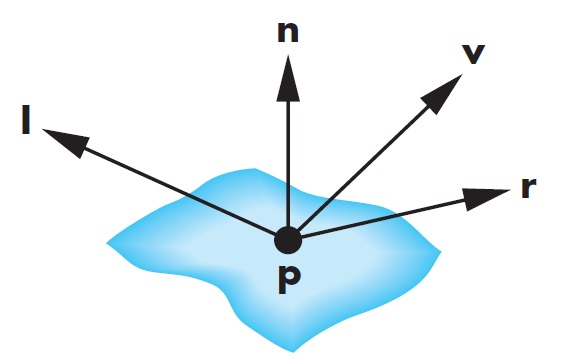
\includegraphics[scale=0.4]{./images/phong-reflection-model-vectors}\\
%%Inputs
		& $p$ is the point where the incident ray $L_{i}$ intersects the 
		object's surface.\\
		& $p_{0}$ is position of the light source. \\				
		& $L_{i}$ is the normalized incident ray hitting point $p$.\\
		\hline
%%Calculated aspects
	\end{tabular}
\end{minipage}

\begin{minipage}{\textwidth}
	\renewcommand*{\arraystretch}{1.5}
	\begin{tabular}{| p{\colAwidth} | p{\colBwidth}|}
		\hline
		\rowcolor[gray]{0.9}
		Number& \iref{IM_Phong} (continued)\\
		\hline
		Label& \bf Phong Reflection Model\\
		\hline
		%Middle calculations
		Description & $N$ is the surface normal at point 
		$p$.\\
		& $k_{d}$ is the diffuse coefficient.\\
		& $k_{s}$ is the specular coefficient\\
		& $\alpha$ : is the shininess coefficient\\		
		& $L_{r}$ is the normalized reflection of $L_{i}$ about $N$.\\
		& $V$ is the normalized vector between the observer and $p$. $V = 
		||$OBSERVER\_POSITION $- p||$\\
		& $I_{a}$ is the ambient intensity of the light described by 
		$L_{i}$ at point $p$. It is described by 
		\ddref{DD_Intensity_ambient} as:\\
		& $I_{d}$ is the diffuse intensity of the light described by 
		$L_{i}$ at point $p$. It is described by 
		\ddref{DD_Intensity_diffuse} as : \\
		& $I_{d} = k_{d} \cdot \max(0, (N \bullet 
		L_{i}))\cdot i(p,p_{0}) \cdot$ OBJECT\_BASE\_COLOUR \\
		& $I_{s}$ is the specular intensity of the light described by 
		$L_{i}$ at point $p$. It is described by 
		\ddref{DD_Intensity_specular} as: \\
		& $I_{s} = k_{s} \cdot \max(0, (L_{r} \bullet V))^\alpha \cdot
		i(p,p_{0})\cdot$ OBJECT\_SPECULAR\_COLOUR \\
		\hline
		Sources& \cite{Comninos2005,Lengyel2003,shreiner2012} \\
		\hline
		Ref.\ By & \iref{IM_Blinn_Phong}\\
		\hline
		Uses & \ddref{DD_Intensity_specular},\ddref{DD_Intensity_diffuse}, 
		\ddref{DD_Intensity_ambient}, \ddref{DD_Intensity_Total}, 
		\ddref{DD_Intensity_PointSource_Distance}, \ddref{DD_Dot_Product} \\
		\hline
	\end{tabular}
\end{minipage}\\

~\newline

\noindent
\begin{minipage}{\textwidth}
	\renewcommand*{\arraystretch}{1.5}
	\begin{tabular}{| p{\colAwidth} | p{\colBwidth}|}
		\hline
		\rowcolor[gray]{0.9}
		Number& IM\refstepcounter{instnum}\theinstnum \label{IM_Blinn_Phong}\\
		\hline
		Label& \bf Blinn-Phong Reflection Model\\
		\hline
		\multirow{12}{*}{Input} & $L_{i}$ : Vector $\langle x, y ,z \rangle$\\
		& $p$ : Point (x,y,z)\\
		& OBSERVER\_POSITION : Point (x,y,z)\\		
		& OBJECT\_POSITION : Point (x,y,z)\\
		& OBJECT\_BASE\_COLOUR : (r,g,b)\\
		& $k_{d}$ : $\mathbb{R}$\\
		& OBJECT\_SPECULAR\_COLOUR: (r,g,b)\\
		& $k_{s}$ : $\mathbb{R}$ \\
		& $\alpha$ : $\mathbb{R}$ \\
		& $N$ : Vector $\langle x, y ,z \rangle$\\
		& $p_{0}$ : Point (x,y,z)\\		
		& LIGHT\_COLOUR : (r,g,b)\\	
		\hline
		\multirow{2}{*}{Output} & $I_{T}$ : (r,g,b)\\
		& OBJECT\_RENDERING\_COLOUR: (r,g,b)\\
		\hline
		Equation & $I_{T} = I_{a} + I_{d} + I_{s}$\\
		& OBJECT\_RENDERING\_COLOUR = $(I_{T})\cdot$(LIGHT\_COLOUR)\\
		Description& The Blinn-Phong model is a modification of the Phong model 
		where calculations use the half-direction vector, $H$. This changes the 
		calculation of $I_{s}$ but nothing else.\\
		&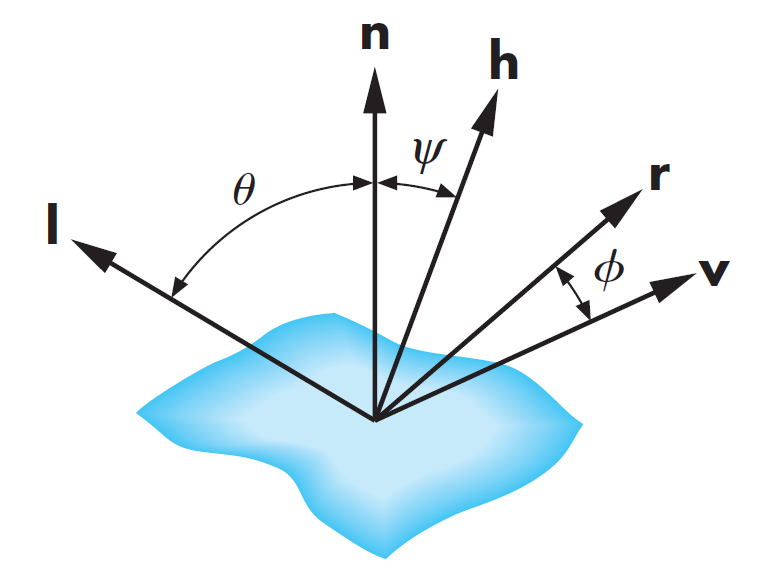
\includegraphics[scale=0.4]{./images/blinn-phong-reflection-model-vectors}\\
		\hline
	\end{tabular}
\end{minipage}\\

\begin{minipage}{\textwidth}
	\renewcommand*{\arraystretch}{1.5}
	\begin{tabular}{| p{\colAwidth} | p{\colBwidth}|}
		\hline
		\rowcolor[gray]{0.9}
		Number& \iref{IM_Blinn_Phong} (continued)\\
		\hline
		Label& \bf Blinn-Phong Reflection Model\\
		\hline
		%Middle calculations
		Description & $p$ is the point where the incident ray $L_{i}$ 
		intersects the 	object's surface.\\
		& $p_{0}$ is position of the light source. \\				
		& $L_{i}$ is the normalized incident ray hitting point $p$.\\
		& $N$ is the surface normal at point $p$.\\
		& $k_{d}$ is the diffuse coefficient.\\
		& $k_{s}$ is the specular coefficient\\
		& $\alpha$ : is the shininess coefficient\\		
		& $L_{r}$ is the normalized reflection of $L_{i}$ about $N$.\\
		& $V$ is the normalized vector between the observer and $p$. $V = 
		||$OBSERVER\_POSITION $- p||$\\
		& $H$ is the half-direction vector between $V$ and $L_{i}$. $H = 
		||V+L_{i}||$\\		
		& $I_{a}$ is the ambient intensity of the light described by 
		$L_{i}$ at point $p$. It is described by 
		\ddref{DD_Intensity_ambient} as:\\
		& $I_{d}$ is the diffuse intensity of the light described by 
		$L_{i}$ at point $p$. It is described by 
		\ddref{DD_Intensity_diffuse} as : \\
		& $I_{d} = k_{d}\cdot max(0, (N \bullet 
		L_{i}))\cdot i(p,p_{0})\cdot$ OBJECT\_BASE\_COLOUR \\
		& $I_{s}$ is the specular intensity of the light described by 
		$L_{i}$ at point $p$. It is described by: \\
		& $I_{s} = k_{s} \cdot \max(0, (N \bullet H))^\alpha \cdot
		i(p,p_{0}) \cdot$ OBJECT\_SPECULAR\_COLOUR \\
		\hline
		Sources& \cite{Comninos2005,Lengyel2003,shreiner2012} \\
		\hline
		Ref.\ By & \iref{IM_Blinn_Phong}\\
		\hline
		Uses & \ddref{DD_Intensity_diffuse}, 
		\ddref{DD_Intensity_ambient}, \ddref{DD_Intensity_Total}, 
		\ddref{DD_Intensity_PointSource_Distance}, \ddref{DD_Dot_Product} \\
		\hline
	\end{tabular}
\end{minipage}\\

~\newline

\subsection{Output} \label{sec_Output}    
\begin{table}[H]
	\centering
	\begin{tabular}{|p{5cm}|p{10cm}|}
		\hline
		\textbf{Variability} & \textbf{Parameter of Variation} \\
		\hline
		Output file & Generated code file that when compiled renders a scene, 
		executable file that shows the rendered scene\\
		\hline
	\end{tabular}
	\caption{Parameters of Variation for Output.}
	\label{tbl:Output_Variations}
\end{table}

\section{Requirements}
This section provides the functional requirements, the business tasks that the
software is expected to complete, and the nonfunctional requirements, the
qualities that the software is expected to exhibit.

\subsection{Family of Functional Requirements}
The following are a list of the services that the system shall provide:
\noindent 
\begin{itemize}
%%Reliability
	\item[R\refstepcounter{reqnum}\thereqnum \label{R_Inputs1}:] When presented 
	with a scene in a file, the system shall correctly read from file the 
	input data for light source(s) and object(s).
	%%Rationale: The system may be provided a file with scene data. I want to 
	%%leave this open that there could be a GUI with dropdown selections to 
	%%make this process easier - ergo the "when".

	\item[R\refstepcounter{reqnum}\thereqnum \label{R_Inputs1Err}:]System 
	responds with specific error message when system cannot read input files.
	
	\item[R\refstepcounter{reqnum}\thereqnum \label{R_Inputs1Err-Def}:]	The 
	system asks user if they would like to use the default settings when scene 
	size, shading model, and/or reflection model information is missing from 
	input, and applies (DEF\_HEIGHT, DEF\_WIDTH, DEF\_DEPTH), DEF\_SHADE and/or 
	DEF\_LIGHT if the user answers yes.
	%%Rationale: The system should be robust enough to render a scene when 
	%%given just the light source, object information. This gives new users 
	%%room to learn the input method. 

	\item[R\refstepcounter{reqnum}\thereqnum \label{R_DefaultScene}:]When no 
	input file is given, the system provides a default scene of dimension 
	(DEF\_HEIGHT, DEF\_WIDTH, DEF\_DEPTH) with one point light source with the 
	default light colour, one sphere with the default material properties, 
	rendered using default shading (DEF\_SHADE) and lighting (DEF\_LIGHT).
	%%Rationale: The system needs a default test case that shows minimum 
	%%functioning.
	
	\item[R\refstepcounter{reqnum}\thereqnum \label{R_Inputs2}:]The system 
	shall verify that all input data meets constraints laid out in Table 
	\ref{tbl:Input_Variations}.

	\item[R\refstepcounter{reqnum}\thereqnum \label{R_Inputs2Err}:] The system 
	responds with specific error message when user inputs contain errors (type 
	mismatch, data outside of constraints).
	
	\item[R\refstepcounter{reqnum}\thereqnum \label{R_Calculate1}:] The library 
	shall correctly calculate the surface normals for object(s) based on 
	shading model.
	 
	\item[R\refstepcounter{reqnum}\thereqnum \label{R_Calculate2}:] The library 
	shall calculate the incidence and reflection vectors off of object(s) 
	surface(s) based on light position(s), object(s) properties, shading model 
	and observer position.
	
	\item[R\refstepcounter{reqnum}\thereqnum \label{R_Calculate3}:] The library 
	shall calculate the light intensity based on light position(s), object(s) 
	material properties, and shading model.
	
	\item[R\refstepcounter{reqnum}\thereqnum \label{R_Calculate4}:] The library 
	shall calculate the final colour object(s) faces based on the intensities 
	calculated in \rref{R_Calculate3}.
	
	\item[R\refstepcounter{reqnum}\thereqnum \label{R_Output}:] The library 
	will output code for a lit and shaded scene.
	
	\item[R\refstepcounter{reqnum}\thereqnum \label{R_Performance}:]Users can 
	render a default scene (define in \rref{R_DefaultScene}) faster than in 
	OpenGL.
	%%Rationale: Performance comparison against main competitor.
\end{itemize}

\wss{I suggest changing the phrasing of the requirements to say the library
  offers these services.}

\subsection{Nonfunctional Requirements}
\noindent 
\begin{itemize}	
%% Productivity Requirements
	\item[R\refstepcounter{reqnum}\thereqnum 
	\label{NFR-Productivity-InputMods}:] 
	The addition of new input methods should not affect the usability of the 
	system.
	%%Rationale: The input methods should be a secret of the system that 
	%%doesn't affect the interface. I'm not sure where to capture this. 
	\item[R\refstepcounter{reqnum}\thereqnum 
	\label{NFR-Productivity-Modifications}:] 
	The addition of new lighting models, shading models, types of light sources 
	and/or types of objects should be completable in 
	MODIFICATION\_TIME\_THRESHOLD.
	%%Rationale: The system should allow for expansion with new approximations; 
	%%the design of the system should allow for new models or types to be 
	%%inserted with minimal effort since all should require the same underlying 
	%%information (object material properties, luminous intensity, etc.) The 
	%%ability to modify the system in a defined amount of time adds to the 
	%%overall productivity of the software as people would be able to expand 
	%%and use it in a minimal amount of time. 
%% Usability Requirements	
	\item[R\refstepcounter{reqnum}\thereqnum \label{NFR-Usability-Install}:] 
	USABILITY\_THRESHOLD \% of users can install the system without requiring 
	assistance.
	%%Rationale: System usability is directly affected by whether it is easy to 
	%%install.
	\item[R\refstepcounter{reqnum}\thereqnum \label{NFR-Usability-load}:] 
	USABILITY\_THRESHOLD \% of users can load an existing scene with no 
	assistance.
	%%Rationale: Usability is determined by ability to perform the basic 
	%%functions without needing assistance/making errors. It's unreasonable at 
	%%this stage to dictate the number of errors that is a threshold since I 
	%%haven't figured out what the system interface is going to look like - so 
	%%the best method of judging at the moment is whether they can perform the 
	%%tasks with no assistance regardless of how long it takes. Future 
	%%refinements of this should indicate how many steps this particular 
	%%interaction should be to quantify this data.
	\item[R\refstepcounter{reqnum}\thereqnum \label{NFR-Usability-changes}:] 
	USABILITY\_THRESHOLD \% of users can change the parameters of the lighting 
	models and re-render an existing scene with no assistance.
	%%Rationale: same as above. The ability to perform this also informs us 
	%%about the user's ability to recover from errors. If they entered the 
	%%wrong model for example, they can enact this ability to correct it.
	\item[R\refstepcounter{reqnum}\thereqnum \label{NFR-Usability-new}:] 
	USABILITY\_THRESHOLD \% of users can initialise a new scene with the 
	default parameters (default object, light source, lighting model, and 
	shader) with no assistance.
	%%Rationale: same as above.		
	\item[R\refstepcounter{reqnum}\thereqnum \label{NFR-Usability-perceived}:] 
	USABILITY\_THRESHOLD \% of users perceive \famname to be easier to use than 
	OpenGL.
	%%Rationale: Way to qualitatively quantify how this system compares to on 
	%%of its competitors.		
	\item[R\refstepcounter{reqnum}\thereqnum 
	\label{NFR-Usability-control-perceived}:] 
	USABILITY\_THRESHOLD \% of users perceive \famname to allow them more 
	control than the built in Unity shader options.
	%%Rationale: Way to qualitatively quantify how this system compares to on 
	%%of its competitors.	
\end{itemize}

\wss{There is an issue on GitHub about the NFRs here mostly being FRs.}

\section{Likely Changes}    

\noindent \begin{itemize}

\item[LC\refstepcounter{lcnum}\thelcnum\label{LC_refraction}:] Refractive 
materials incorporated into family.
\item[LC\refstepcounter{lcnum}\thelcnum\label{LC_reflection_models}:] More 
reflection models incorporated into family.
\item[LC\refstepcounter{lcnum}\thelcnum\label{LC_normals}:] Variations on how 
normals are computed (e.g. partial derivatives) may be added to the family.

\end{itemize}

\section{Traceability Matrices and Graphs}
	\begin{table}[H]
		\begin{tabular}{|l||l|l|l|l|l|l|l|l|l|l|l|}
			\hline
			& \aSref{as-geometrical_appx} & \aSref{as-illumination} & 
			\aSref{as-loc-vs-global} & \aSref{as-illum_constraint} & 
			\aSref{as-emission_constraint} & \aBref{as-coordinate_system} & 
			\aBref{as-coordinates} & \aBref{as-obsv_total} & 
			\aBref{as-object_representation} & 
			\aBref{as-object_representation2} & \aBref{as-object_refraction} \\
			\hline
			\tref{TM_Reflection} & X & & & & X & X & & & & & X \\
			\hline
			\dref{GD_diffReflect} & X & & X & & X & X & & & & & \\
			\hline
			\iref{IM_LamDiffuse} &X&X&X&X&X& & & & & &\\
			\hline
			\iref{IM_HalfLam} &X&X&X&X&X& & & & & & \\
			\hline
			\iref{IM_Phong} & X&X&X&X&X& &X&X& & & \\
			\hline
			\iref{IM_Blinn_Phong}& X&X&X&X&X& &X&X& & & \\
			\hline
			\ddref{DD_Dot_Product} & & & & & &X&X& & & & \\ 
			\hline
			\ddref{DD_Cross_Product} & & & & &&X&X& & & & \\		
			\hline
			\ddref{DD_Intensity_ambient} &X&X&X&X& & & & & & & \\
			\hline
			\ddref{DD_Intensity_diffuse} & &X& & &X& & & & & &X\\
			\hline
			\ddref{DD_Intensity_specular}& &X& & &X& & & & & &X\\			
			\hline
			\ddref{DD_Intensity_Total} & &X&X&X&X& & & & & &X\\		
			\hline
			\ddref{DD_Intensity_PointSource_Distance} &X&X& & & &X&X& & & & \\
			\hline
			\ddref{DD_Flat_Shading} &X& && &X&X&X& &X& & \\
			\hline
			\ddref{DD_Gouraud_Shading} &X&X&X&&X&X&X& &X&X&X\\			
			\hline
			\ddref{DD_Phong_Shading} &X&X&X&&X&X&X& &X&X&X\\			
			\hline
			\lcref{LC_normals} &X& & & & &X&X& &X&X& \\			
			\hline
			\lcref{LC_reflection_models} & &X&X&X&X& &X& & & 
			&X\\						
			\hline
			\lcref{LC_refraction} & &X&X&X&X& & & & & &X\\
			\hline						
		\end{tabular}
		\caption{Traceability Matrix matching Scope and Build Time Assumptions 
		to Theoretical Models, General Definitions, Instance Models, Data 
		Definitions and Likely Changes.}
	\end{table}	

\section{Appendix}

\subsection{First Stage of Implementation}
%\plt{In this section specify the family member, or sub-family, that you will be
%	implementing for CAS 741.  You should specify the value for all of your
%	variabilities, along with the binding time.  A tabular representation will
%	probably be the easiest way to convey this information.}

In this project I aim to implement the local illumination shading and lighting 
models outlined in this document. This means I've invoked 
\aref{as-geometrical_appx}, \aref{as-illumination} and will only be working 
with members of the family outlined in this document. The overall goal is to 
implement these shaders as plug-ins for Unity (a game development engine), as 
such I have made certain build-time decisions to fit this context.

The following table illustrates the build-time decisions that I've made to 
scope the project further.
\begin{table}[H]
	\begin{tabular}{|p{4cm}|p{8cm}|p{2.4cm}|}
		\hline
		\textbf{Variability} & \textbf{Decisions} & 
		\textbf{Related Assumptions}\\
		\hline
%%Input Structure
		\multirow{4}{*}{Input} & Input file will be formatted JSON, using 
		standard conventions & \\
		& Files will be stored in SCENE\_DIR & \\
		& File contents can be modified by the user from the system GUI, 
		the changes will be stored as proper JSON information & \\
		& Files will list information in the following order:
		\begin{itemize}
			\item scene size;
			\item lighting model;
			\item shading model;
			\item light source information;
			\item object information;
			\item observer information;			
		\end{itemize}	& \\
		\hline
	\end{tabular}
\end{table}

\begin{table}[H]
	\begin{tabular}{|p{4cm}|p{8cm}|p{2.4cm}|}
		\hline
		\textbf{Variability} & \textbf{Decisions} & 
		\textbf{Related Assumptions}\\
		\hline
%%System Internals
%Coordinate System
		\multirow{2}{*}{Coordinate System} & 3D Cartesian Coordinates with 
		right-hand rules. & 
		\aref{as-coordinate_system}\\ 
		& System coordinates will be handled with floating point numbers. & \\	
		\hline
%Scene
		\multirow{4}{*}{Scene} & Scene size will be ordered as (height, width, 
		depth) & 
		\aref{as-scenes-size} \\
		& Scene size can be passed in at run-time through file & \\
		& Default scene size will be (DEF\_HEIGHT, DEF\_WIDTH, DEF\_DEPTH) & \\
		& Only one scene is loaded at a time. & \aref{as-number-scenes} \\
		\hline
%Lighting Model
		Lighting Model & Lighting model can be one of: \iref{IM_LamDiffuse}, 
		\iref{IM_HalfLam}, \iref{IM_Phong}, \iref{IM_Blinn_Phong} & \\
		\hline
%Shading Model
		Shading Model & Shading model can be one of: \ddref{DD_Flat_Shading}, 
		\ddref{DD_Gouraud_Shading}, \ddref{DD_Phong_Shading} & \\
		\hline
%Lights
		\multirow{3}{*}{Lights} & Lights can be point lights, spotlights, 
		directional lights, or ambient lights & \\
		& Light can be passed in at run-time through file. & \\
		& Light structures will contain the type of light, the colour of the 
		light, the position of the light,  & 
		\\
		\hline
%Objects
		\multirow{3}{*}{Objects} & Objects can be spheres, cubes, toruses, or 
		teapot & \\
		& Objects can be passed in at run-time through file. & \\
		& Object structures will contain a mesh containing a list of vertices 
		and surfaces associated with vertices, the centrepoint of the object, 
		and the material properties of the object (base colour, specular 
		colour, coefficient of diffuse, specular, and ambient reflections, 
		coefficient of shininess) & \\
		& Objects will all have a white specular colour (255,255,255) & \\
		\hline
	\end{tabular}
\end{table}

\begin{table}[H]
	\begin{tabular}{|p{4cm}|p{8cm}|p{2.4cm}|}
		\hline
		\textbf{Variability} & \textbf{Decisions} & 
		\textbf{Related Assumptions}\\
		\hline
		%Observer
		\multirow{3}{*}{Observer} & There can only be 1 observer in a scene. &	
		\\
		& Observer information can be passed in at run-time through a file & \\
		& Observer structure contains a position (x,y,z) that it is located at, 
		and a direction that it is facing. & \\
		\hline		
		%%Output Structure
		\multirow{2}{*}{Output} & Output will be a rendered scene using the 
		Unity Engine & \\
		& Rendered output image will be saved as an Unity executable in the 
		director RENDERS\_DIR & \\
		\hline		
	\end{tabular}
\end{table}

We prioritize the implementation of the default scene's shading (DEF\_SHADE) 
and lighting model (DEF\_LIGHTS). 

\wss{I think we need more information than this.  What are the values of the
  variabilities in your table?  For instance, what objects are you allowing?}


\newpage

\bibliographystyle {plainnat}
\bibliography {../refs/References}

\newpage

\end{document}